\newpage
\chapter{ANALİTİK ÖNGÖRÜLER VE SİMÜLASYONLAR}\label{ch:simulasyonlar}
\paragraph{}
Bu tezde altı adet ana simülasyon modelinin sonucu incelenmiştir. Simülasyonların isimlendirilmesi, dikkate alınan etkileşimler ve potansiyellerin konum bağımlılıkları \ref{tab:simulasyonlar} numaralı tabloda yer almaktadır. Simülasyon modelleri, oyuncak model ve gerçekçi model olarak ikiye ayrılmıştır. Oyuncak modeller etkileşim potansiyellerinin analitik formülleri kullanılarak yapılırken, gerçekçi modellerde ÇÇSN simülasyonundan elde edilen sayısal baryon profili kullanılmıştır. 

Öncelikle, oyuncak modeller başlığı altında madde profilinin analitik ifadesi bilinen bir potansiyel için simülasyonlar yapılacaktır. Eksponansiyel olarak azalan madde profili ve $ (50 \text{ km}/r)^{2} $ ile azalan manyetik alan profili altında analitik öngörüler ile sayısal sonuçlar karşılaştırılacaktır. Sonuçları daha iyi anlayabilmek için önce karışım açısının sıfır olduğu, yani boşluk salınımlarının olmadığı durumda, hem analitik hem de sayısal elektron nötrino yaşama olasılıkları elde edilecektir. Ardından küçük bir çeşni karışım açısı altında sonuçların değişimine bakılacaktır. Tüm bunlar \ref{sec:OyuncakModel} numaralı bölümde incelenecektir.

Oyuncak modeller incelendikten sonra \ref{sec:gercekciModeller} numaralı bölümde ÇÇSN'nin gerçekçi madde profili kullanılarak çeşni evrimi incelenecektir. Gerçekçi modeller için \cite{1987ESOC...26..325N} numaralı kaynaktan ön süpernova (pre-supernova) modeli alınıp üzerine şok dalgası eklenmiştir. Şok dalgası ise \cite{Athar:1995cx} numaralı kaynaktaki parametrizasyon yardımı ile madde profiline eklenmiştir.

Gerçekçi modeller için de dört farklı simülasyon yapılmıştır. Simülasyonlarda nötrino öz-kırılımı ve nötrino manyetik alan etkileşiminin kollektif çeşni salınımlarına olan etkisi incelenmiştir. Simülasyonların adlandırılması \ref{tab:simulasyonlar} numaralı tabloda verilmiştir.

\begin{table}[hbt!]
    \centering
    \begin{tabular}{|c|c|c|}
        \hline
         & \textbf{Etkileşimler} & \textbf{Potansiyeller} \\ 
        \hline
        \small{theta0expNbB}   & $M,EM$  & \footnotesize{$n_{b}(r)=10^{6} e^{-r/200 \text{ km}} $ [g/cm$^{3}$], $B\approx 10^{15} \qty(\frac{50 \text{ km}}{r})^{2}$  [Gauss]}\\
        \hline
        \small{theta014expNbB} & $\nu,M,EM$  & \footnotesize{$n_{b}(r)=10^{6} e^{-r/200 \text{ km}} $ [g/cm$^{3}$], $B\approx 10^{15} \qty(\frac{50 \text{ km}}{r})^{2}$  [Gauss]}\\
        \hline
        \small{t5sNoCollnuNoB}  & $\nu,M$ & \cite{1987ESOC...26..325N, Athar:1995cx} kaynaklarından $ t=5 $s için $n_{b}(r)$\\
        \hline
        \small{t5sNoCollnuB}   & $\nu,M,EM$  &\tiny{\cite{1987ESOC...26..325N, Athar:1995cx} kaynaklarından $ t=5 $s için $n_{b}(r)$ ve $B= 10^{15} \qty(\frac{50 \text{ km}}{r})^{2}$ [Gauss]}\\
        \hline
        \small{t5sCollnuNoB}   & $\nu,M,\nu\nu$ &\cite{1987ESOC...26..325N, Athar:1995cx} kaynaklarından $ t=5 $s için $n_{b}(r)$\\
        \hline
        \small{t5sCollnuB}     & $\nu,M,EM, \nu\nu$ &\tiny{\cite{1987ESOC...26..325N, Athar:1995cx} kaynaklarından $ t=5 $s için $n_{b}(r)$ ve $B= 10^{15} \qty(\frac{50 \text{ km}}{r})^{2}$ [Gauss]}\\
        \hline
    \end{tabular}
    \caption[Simülasyon Adlandırılması, Etkileşimler Ve Potansiyeller.]{\label{tab:simulasyonlar}Simülasyon adlandırılması, dikkate alınan etkileşimler ve potansiyellere ait profiller. theta014expNbB adlı modelde, baryon profilinin başlangıçtaki değeri olan $ 10^{6} $ g/cm$^{3}$ değeri ÇÇSN $t=5$ s için olan profilin fit değeridir. Bu modelin altında, başlangıç baryon yoğunluğu farklı olan alt simülasyonlar da yapılmıştır. Ayrıca, theta014expNbB modeli incelenirken normal hiyerarşi ve elektron antinötrino kutu spektrumuna sahip simülasyonlar da yapılmıştır. Manyetik alan profilleri \cite{deGouvea:2012hg,deGouvea:2013zp,Kharlanov:2020cti} numaralı referanslarla uyumludur.}
\end{table}

\section{ANALİTİK ÖNGÖRÜLER}\label{sec:evrim}
\paragraph{}
Bu bölümde, yapılacak olan simülasyonların hareket denklemlerini, özbazdaki ortalama çözümleri ve geçiş olasılıklarını inceleyeceğiz.  Yoğunluk operatörünün başlangıçtaki ifadesi aşağıdaki gibi yazılır.
\begin{align}
    \nonumber \hat{\rho}(R) =& \sum_{i,j} \mel{E_{i}(R)}{\hat{\rho}}{E_{j}(R)} \dyad{\Psi_{i}(R)}{\Psi_{j}(R)} \text{ ,}\\
    = & \sum_{i,j} \rho_{ij}(R) \dyad{\Psi_{i}(R)}{\Psi_{j}(R)} \text{ .}
\end{align}
Burada $ \ket{E_{i}(R)} $ sistemin başlangıçtaki özvektörü, $ \Psi_{i}(R) $ ise nötrinoların başlangıçtaki durum ketidir. Bu çalışmada, aksi belirtilmedikçe başlangıç nötrino durum keti, ya sadece elektron nötrino olarak ya da sadece elektron antinötrinosu olarak tanımlanacaktır. Yoğunluk operatörünü herhangi bir uzaklıktaki ifadesini yazmak için durum ketini evrimleştirmek gerekmektedir.
\begin{equation}\label{eqn:psiAexp}
    \ket{\Psi_{i}(r)} = \sum_{a} A^{\dagger}_{ia}(r) \exp(-i\int^{r}_{R} E_{a}(x) \dd{x}) \ket{E_{a}(r)} \text{ .}
\end{equation}
$ A $ matrisi, evrimin adyabatikliğini belirleyen, \eqref{eqn:LZamplitude} numaralı denklemde tanımlanan, özvektörler arasındaki geçişi veren LZ geçiş genlik matrisidir. 

Nötrinolar evrimlerini bir özbazda başlayıp bitirebilir. Bu durum, başlangıçtaki özbazda yazılan yoğunluk matrisinin, köşegen elemanlarının değişmeden aynı kalması anlamına gelir. Bir önceki bölümde bu çeşit evrime adyabatik evrim adı verilmişti. Bir diğer taraftan, nötrinolar belli bir uzaklığa geldiğinde, o uzaklıktaki özvektörler, başlangıçtaki özvektörlerin bir süper pozisyonu olabilir. Bu durum da adyabatiklikten sapma olarak belirtebiliriz. Son olarak özvektörler yer değiştirebilir. Bu da evrimin diabatik olduğu anlamına gelir.

\eqref{eqn:psiAexp} numaralı denklemde $ E_{a}(r) $, sistemin $ r $ uzaklığındaki özdeğerleridir. Tüm eksponansiyel terim evrimin salınım fazını oluşturur. Yoğunluk operatörü, $ r $ uzaklığına geldiğinde 
\begin{align}
    \nonumber \hat{\rho}(r) =& \sum_{a,b}\sum_{i,j} \qty(A_{ai}(r) \rho_{ij}(R) A^{\dagger}_{jb}(r))\exp(-i\int^{r}_{R} \qty(E_{a}(x)- E_{b}(x)) \dd{x})\\ 
    \nonumber &\times \dyad{E_{i}(r)}{E_{j}(r)} \text{ ,} \\
    =& \sum_{a,b}\sum_{i,j}\qty(A_{ai}(r) \rho_{ij}(R) A^{\dagger}_{jb}(r)) C_{ij}(E)
    \dyad{E_{i}(r)}{E_{j}(r)} \text{ ,}
\end{align}
şeklinde olacaktır. Evrime gelen salınım fazı, $ C_{ij}(E) $, sadece enerji özdeğerlerine bağlıdır. Bu faz çeşni bazında yazılan yaşama olasılığında ortalama bir değer üzerinde salınıma sebep olur. Yoğunluk operatörünü ortalama kısmı, $ \hat{\bar{\rho}}(r) $, ve salınan kısmı, $ \hat{\rho}_{sal}(r) $, olarak iki şekilde yazabiliriz.
\begin{align}\label{eqn:rhoBar_rhoSal}
    \nonumber \hat{\rho}(r) = & \hat{\bar{\rho}}(r) + \hat{\rho}_{sal}(r) \text{ ,}\\
    \nonumber               = &   \sum_{a}\sum_{i,j}\qty(A_{ai}(r) \rho_{ij}(R) A^{\dagger}_{ja}(r)) \dyad{E_{i}(r)}{E_{j}(r)} \\
                              & + \sum_{\substack{a,b\\ a \ne b}}\sum_{i,j}\qty(A_{ai}(r) \rho_{ij}(R) A^{\dagger}_{jb}(r)) C_{ij}(E) \dyad{E_{i}(r)}{E_{j}(r)} \text{ .}
\end{align}

Yoğunluk operatörün ortalama kısmı evrim hakkında genel bir fikir vermemizi sağlar. Özellikle çok uzaklardan gelen kaynaklarda, na-eş evreli (decoherance) kaynaklı çeşni salınım kısmı sıfıra inecektir \cite{GIUNTI199287, Hansen:2016klk}. Çeşni evrimi sırasında nötrinolar, bir özbazdan başka bir özbaza atlarsa salınımların etkisi ortaya çıkacaktır. 

Özdurumların yerine tedirgeme teorisinden elde ettiğimiz \eqref{eqn:EMbasisKets} numaralı ifadeleri koyabiliriz. Bu durumda yoğunluk operatörünün çeşni tabanındaki ifadesini yaklaşık olarak elde edebiliriz. Ortalama yoğunluk operatörünün $ ee $ tabanına izdüşümü, adyabatik bir evrim için aşağıdaki gibi verilir.
\begin{align}
    \nonumber\rho_{ee}(r)  =& \sum_{i} \rho_{ii}(R) \braket{\nu_{e}}{\nu_{i}^{EM}(r)} \braket{\nu_{i}^{EM}(r)}{\nu_{e}} \\
    \nonumber=& \frac{\rho_{11}(R) c^{2}_{\theta_{M}}}{N^{2}_{1}}+ \frac{\rho_{22}(R) s^{2}_{\theta_{M}}}{N^{2}_{2}}+ \frac{\rho_{33}(R) \mu^{2} B^{2}}{N^{2}_{3}} \qty(\frac{s_{\gamma} c_{\theta_{M}}}{\delta \omega_{31}}+\frac{c_{\gamma} s_{\theta_{M}}}{\delta \omega_{32}})^{2}\\
    &+ \frac{\rho_{44}(R) \mu^{2} B^{2}}{N^{2}_{4}} \qty(\frac{c_{\gamma} c_{\theta_{M}}}{\delta \omega_{41}}+\frac{s_{\gamma} s_{\theta_{M}}}{\delta \omega_{42}})^{2}
\end{align}
Burada LZ geçiş genlik matrisi $ A $, birim matris olarak tanımlanarak adyabatik evrim varsayılmıştır.

Nötrinoların içerisinden geçtiği ortam çok ani değiştiğinde veya bir süreksizlik meydana geldiğinde evrim bir özbazdan başka bir özbaza geçecektir. Bu yeni özbaz evrimin geri kalanından sorumlu olacak ve çeşni evrimini belirleyecektir. Bu örnek, iki farklı başlangıç koşulu ve iki farklı simülasyonun birleştirilmesi olarak düşünülebilir. Bu süreksizliğin olduğu noktanın öncesindeki ve sonrasındaki yoğunluk operatörlerinin birleştirilmesi gerekmektedir.

Yukarıda bahsedilen süreksizlik, elektron kesrinin ani değişmesinden kaynaklanabilir. ÇÇSN oluşmadan önce ve oluştuğu ilk saniyelerde elektron kesrinin belli bir $ r_{d} $ değerinde çok hızlı değişmesi gerektiği düşünülmektedir \cite{Athar:1995cx}. Bu değerden kaynaklı çeşni evriminde bir süreksizlik meydana gelecektir. 

Ani değişimin yaşandığı $ r_{d} $ uzaklığının öncesindeki özvektörlere $ \ket{E_{i}} $, sonrasındaki özvektörlere de $ \ket{E'_{i}} $ adını verelim. Basitlik olması açısından, nötrinoların arka planda meydana gelen ani değişime kadar ve ani değişimden sonraki evrimi adyabatik olsun. Yani LZ geçiş matrisi, $ A(r) $, süreksizlikten önce ve sonra birim matris olsun. Bu durumda yoğunluk operatörü $ r_{d} $ uzaklığına kadar aşağıdaki gibi yazılır.
\begin{align}
    \nonumber \hat{\rho}(r) = \sum_{i,j,k,l} \qty[\rho_{ij}(R) C_{ij}(E) C'_{kl}(E)]~ \dyad{E'_{k}(r)}{E'_{l}(r)} \\
    \times \dyad{E'_{k}(r)}{E_{i}(r_{d})} \dyad{E_{j}(r_{d})}{E'_{l}(r)} \text{ .}
\end{align}
Burada $ C'_{kl} = \exp(-i\int^{r}_{r_{d}} \qty(E'_{k}(x)- E'_{l}(x)) \dd{x}) $ şeklindedir. Ani değişim yaklaşıklığında, Hamiltonyen aniden değiştiğinde, yoğunluk operatörünün evrimi aniden değişmiyor veya değişmek için yeterli zamanı olmuyor \cite{messiah2014quantum}. Süreksizlikten sonra $ C_{ij}(E) $ terimi salınım yapmayı bırakır. Süreksizlik noktasına kadar gelen salınım fazına \emph{donmuş faz} (frozen phase) adı verilecektir. Çeşni bazına geçtiğimizde donmuş fazın bilgisi, $ r_{d} $ uzaklığından sonra da kalır. Donmuş faz nedeniyle salınan yaşama olasılığı, $ r_{d} $ değerine geldiğinde bambaşka bir faz ile salınmaya başlar. İşte bulduğumuz bu donmuş fazın varlığı ve $ r_{d} $ noktasındaki değeri, süreksizlikten sonra da etkisini göstermektedir. Öte yandan $ C'_{kl}(E) $ salınım fazı, süreksizlik noktasından sonra kazandığı fazdır ve bir ortalamanın etrafında salınır. Eğer ikinci bir süreksizlik yoksa $ C'_{kl}(E) $ fazı sadece salınım terimlerini verecektir. 

Süpernova ortamında elektron kesrinin süreksizliği gibi baryon kütlesinin süreksizliği de oluşmaktadır. Bu süreksizliği yaratacak olan en büyük değişim şok dalgasının ön yüzü olacaktır. Şok dalgasının, süpernova merkezinden dışarı doğru bakan bölümü yani ön yüzündeki değişim nötrinoların çeşni evrimini etkiler ancak yukarıda bahsedildiği gibi bir değişme sebep olmaz. Gerçekçi modeller bölümünde bu konu daha ayrıntılı incelenecektir.

Donmuş fazların etkisine ve çeşni evrimine daha ayrıntılı bakabilmek için yoğunluk operatörünü çeşni tabanında yazmak gerekmektedir. ÇÇSN'nin iç kısımlarına baktığımızda manyetik moment etkisiyle $ e-\bar{x} $ veya $ x-\bar{e} $ geçişleri olabilir. Sadece $ e-\bar{x} $ geçişleri dikkate alındığında enerji özdurumlarından $ \ket{E_{1,2}} $ ve $ \ket{E'_{1,2}} $ baskındır. O halde iki duruma indirgenmiş yoğunluk matrisi aşağıdaki gibi yazılır.
\begin{equation}
    \hat{\overline{\rho}}(r) = \sum^{2}_{i,j,k} C_{ij}(E) \rho_{ij}(R) ~\dyad{E'_{k}(r)}{E_{i}(r_{d})} \dyad{E_{j}(r_{d})}{E'_{k}(r)} \dyad{E'_{k}(r)}{E'_{k}(r)} \text{ .}
\end{equation}
Burada $ k=l $ şeklide alındığı için $C'_{kl} $ terimi atılmıştır. Madde arka planın çok büyük olduğu bir ortamda özvektörler neredeyse çeşni tabanındadır. Bunu, nötrinoların salınım yapamadan madde ile etkileşerek sürekli çeşni tabanında olmaya zorlanması gibi görülebilir. Bu çalışmada genelliği bozmamak için özvektörleri iki farklı çeşninin süperpozisyonu olarak alacağız. Başlangıçta, manyetik alan güçlü olduğundan dolayı özdurumlar çeşni tabanından bir miktar sapabilir. Bundan dolayı şunu yazabiliriz.
\begin{align}
    \ket{E_{1}(r_{d})} =& \cos{\theta_{EM}(R)} \ket{\nu_{\bar{x}}} + \sin{\theta_{EM}(R)} \ket{\nu_{e}} \text{ ,} \\
    \ket{E_{2}(r_{d})} =&-\sin{\theta_{EM}(R)} \ket{\nu_{\bar{x}}} + \cos{\theta_{EM}(R)} \ket{\nu_{e}} \text{ ,} \\
    \ket{E'_{1}(r)} =& \cos{\theta_{EM}(r)} \ket{\nu_{\bar{x}}} + \sin{\theta_{EM}(r)} \ket{\nu_{e}}    \text{ ,} \\
    \ket{E'_{2}(r)} =&-\sin{\theta_{EM}(r)} \ket{\nu_{\bar{x}}} + \cos{\theta_{EM}(r)} \ket{\nu_{e}} \text{ .}
\end{align}
Cebirsel işlemler yapıldığında öz tabanındaki yoğunluk operatörü, çeşni tabanında yazılabilir.
\begin{align}
    \nonumber \hat{\overline{\rho}}(r) = &\qty(\alpha_{11}\cos^{2}\theta_{EM}(r) + \alpha_{22}\sin^{2}\theta_{EM}(r) ) \dyad{\nu_{\bar{x}}}{\nu_{\bar{x}}} \\
    \nonumber &+ \qty(\alpha_{11}\sin^{2}\theta_{EM}(r) + \alpha_{22}\cos^{2}\theta_{EM}(r) ) \dyad{\nu_{e}}{\nu_{e}} \\
    &+ \qty(\alpha_{11}\sin{2\theta_{EM}(r)} - \alpha_{22}\sin{2\theta_{EM}(r)} ) \qty(\dyad{\nu_{e}}{\nu_{\bar{x}}} + \dyad{\nu_{\bar{x}}}{\nu_{e}})  \text{ .}
\end{align}
Burada $ \alpha_{11} $ ve $ \alpha_{22} $ aşağıdaki gibi tanımlanır.
\begin{align}
    \nonumber \alpha_{11} =& \rho_{11}(R)\cos^{2}\qty(\theta_{EM}(R) - \theta_{EM}(r)) \\
    \nonumber             &+ \rho_{22}(R)\sin^{2}\qty(\theta_{EM}(R) - \theta_{EM}(r)) \\
                &+ \rho_{12}\frac{C_{12}+C_{21}}{2}\sin\qty(2\qty(\theta_{EM}(R) - \theta_{EM}(r))) \text{ ,}\\
    \nonumber \alpha_{22} =&-\rho_{11}(R)\sin^{2}\qty(\theta_{EM}(R) - \theta_{EM}(r)) \\
    \nonumber &+ \rho_{22}(R)\cos^{2}\qty(\theta_{EM}(R) - \theta_{EM}(r)) \\
                &- \rho_{12}\frac{C_{12}+C_{21}}{2}\sin\qty(2\qty(\theta_{EM}(R) - \theta_{EM}(r))) \text{ .}
\end{align}

Elde edilen sonuçlar, $ 2\times2 $'ye indirgenebilen $ 1-4 $ Hamiltonyen'i için ve adyabatik evrim varsayımı altında türetilmiştir. Dört çeşni için yaklaşık çözümler tedirgeme kuramından elde edilen özvektörler kullanılarak yazılır.

Geçiş matrisini birim matristen farklı aldığımızda, nötrino yaşama olasılıklarına LZ geçiş olasılıkları dahil olacaktır. Bu sefer LZ geçiş olasılıklarını sisteme dahil ederken salınım terimi $ C_{ij} $ terimi ortalamaya girmez. İki çeşniye indirgenmiş ortalama yoğunluk operatörü \eqref{eqn:rhoBar_rhoSal} numaralı denklem kullanılarak aşağıdaki gibi yazılır.
\begin{align}
    \nonumber \hat{\bar{\rho}}(r) =& \big[(1-P_{LZ})\rho_{11}(R)+P_{LZ}\rho_{22}(R) \\
    \nonumber & ~~ -\qty(e^{i\varphi}\rho_{12}+e^{-i\varphi}\rho_{21}(R)) \sqrt{P_{LZ}(1-P_{LZ})}\big] \dyad{E_{1}(r)}{E_{1}(r)} \\
    \nonumber & \big[P_{LZ}\rho_{11}(R)+(1-P_{LZ})\rho_{22}(R) \\
    & ~~ +\qty(e^{i\varphi}\rho_{12}+e^{-i\varphi}\rho_{21}(R)) \sqrt{P_{LZ}(1-P_{LZ})}\big] \dyad{E_{2}(r)}{E_{2}(r)} \text{ .}
\end{align}
Burada $ \varphi $ terimi Stokes fazdır ve özvektörlerin birbirine geçmesinden gelir. Matematiksel olarak düşünürsek, geçiş genliği $ A $ matrisinin sanal tanımlı olmasından kaynaklıdır. Stokes fazı, aşağıdaki koşul sağlandığında evrimde kendini göstermeyecektir.
\begin{equation}\label{eqn:phaseDisapearCond}
    \frac{(1-P_{LZ}) \rho_{11}(R) + P_{LZ} \rho_{22}(R)}{\sqrt{P_{LZ}(1-P_{LZ})}\rho_{12}(R)} \gg 1 \text{ .}
\end{equation}
LZ geçiş olasılık formülü, \ref{ch:Rezonanslar} bölümünde elde edilirken üç adet yaklaşımdan bahsedilmişti. \eqref{eqn:phaseDisapearCond} numaralı denklemdeki koşul, ikinci yaklaşıklığın sağlanmadığı durumlarda geçerli olur. Yani başlangıçta durum keti Hamiltonyen'in özdurumunda değilse yaşama olasılığına Stokes fazları gelecektir. Başlangıç koşullarında yapılan küçük değişiklikler ise çeşni evriminin son halinde farklılıklara sebep olacaktır. \ref{sec:OyuncakModel} numaralı bölümde, 9 farklı başlangıç koşulu alınarak fazlardan kaynaklanan değişim gösterilecektir.

SFP rezonansının adyabatik olmaması gibi MSW rezonansı da adyabatik olmayabilir. Bu durumda $ A $ matrisi iki farklı rezonans matrisinin çarpımı olacaktır. Bu tezde, aksi belirtilmedikçe, ters hiyerarşi ve $ Y_{e}<0.5 $ değeri göz önüne alındığından dolayı $ A $ matrisini oluşturan LZ rezonans geçiş matris çarpım sırası aşağıdaki gibi olur.
\begin{align}
    \nonumber A =& A_{SFP} \times A_{MSW} \text{ ,}\\
      =& \mqty(\sqrt{1-P_{SFP}} & -e^{-i\alpha}\sqrt{P_{SFP}} & 0 & 0 \\
      e^{i\alpha}\sqrt{P_{SFP}} & \sqrt{1-P_{SFP}} & 0 & 0 \\ 0 & 0 & 1 & 0 \\ 0 & 0 & 0 & 1) \times
      \mqty(1 & 0 & 0 & 0 \\ 0 & \sqrt{1-P_{MSW}} & -e^{-i\beta}\sqrt{P_{MSW}} & 0 \\ 0 & e^{i\beta}\sqrt{P_{MSW}} & \sqrt{1-P_{MSW}} & 0 \\ 0 & 0 & 0 & 1) \text{ .}
\end{align}
Burada $ A_{SFP} $ matrisi $ P_{SFP} $ geçiş olasılıkları ve $ \alpha $ fazına sahiptir. $ A_{MSW} $ matrisi ise $ P_{MSW} $ ve $ \beta $ fazına sahiptir. Bu denklem ancak ve ancak SFP ve MSW rezonansları birbirlerinden "yeterince" ayrı olduklarında doğrudur. Rezonansların birbirlerinden ne kadar ayrıldığı  \ref{sec:OyuncakModel} numaralı bölümde belirlenecektir. 

Geçiş genliğini \eqref{eqn:rhoBar_rhoSal} numaralı denklemde yerine koyup tüm elemanları açık açık yazabiliriz. Bu işlemi yaparken salınım fazı $ C_{ij}(E) $ terimini ise katacağız. Yani geçiş matrislerini sırayla ekleyeceğiz.
\begin{align}
    \rho_{ij}(R)C_{ij}(E) \rightarrow& A^{\dagger}_{SFP}\rho_{ij}(R)C_{ij}(E)~A_{SFP}\\
    \rightarrow& A^{\dagger}_{SFP} ~ \rho_{ij}(R)C_{ij}(E)~A_{SFP} C'_{ij}(E)\\
    \rightarrow& A^{\dagger}_{MSW}A^{\dagger}_{SFP}~\rho_{ij}(R)C_{ij}(E)~A_{SFP} C'_{ij}(E)~A_{MSW} \text{ .}
\end{align}
Denklemleri bu şekilde kurduğumuzda donmuş fazlar dahil neredeyse tüm fazları yoğunluk operatörüne koyuyoruz. Tek dahil etmediğimiz faz, en uzakta meydana gelen MSW rezonansından sonra ortalamaya gelen salınım fazıdır.

Denklemlerin açık ifadesini yazarken ortalama yoğunluk operatörünün öz tabandaki halini üç terime ayıracağız. Bunlardan birincisi ortalama değer, $ \hat{\overline{\rho}}_{\text{ort}} $ olacaktır. İkincisi ise ortalama değerden sapma yani fazlardan kaynaklanan fark olacaktır. Bu terimdeki fazlar başlangıç koşullarına çok hassas şekilde bağlı olduğu için Dünya'da gözlemlenecek her bir nötrino için farklı olacaktır. Bu nedenle kendini bir çeşit ölçüm hatası (error bar) gibi gösterecektir. Biz buna analitik öngörünün \emph{hatası} olarak adlandıracağız ve $ \hat{\overline{\rho}}_{\text{hata}} $ olarak göstereceğiz. Son olarak ortalama etrafındaki salınımları veren köşegen olmayan terimler olacaktır. Bu terime de $ \hat{\overline{\rho}}_{\text{naKos}} $ adı verilecektir. Ortalama yoğunluk operatörü,
\begin{equation} \label{eqn:ortYogun1}
    \hat{\overline{\rho}}(r) = \hat{\overline{\rho}}_{\text{ort}}(r) + \hat{\overline{\rho}}_{\text{hata}}(r) + \hat{\overline{\rho}}_{\text{naKos}}(r) \text{ ,}
\end{equation}
şeklinde yazabiliriz. Bu terimlerden ortalama terim aşağıdaki gibi yazılır.
\begin{align}\label{eqn:rhoBar_ort}
    \nonumber\hat{\overline{\rho}}_{\text{ort}}=& \bigg[(1-P_{SFP}) \rho_{11}(R)+ P_{SFP} \rho_{22}(R)\bigg] \dyad{E_{1}(r)}{E_{1}(r)}\\
    \nonumber&+ \bigg[\qty(1-P_{MSW})\qty(P_{SFP}\rho_{11}(R) +(1-P_{SFP})\rho_{22}(R))\\
    \nonumber&~~~+ P_{MSW} \rho_{33}(R)\bigg] \dyad{E_{2}(r)}{E_{2}(r)}\\
    \nonumber&+ \bigg[P_{MSW}\qty(P_{SFP}\rho_{11}(R)+ (1-P_{SFP})\rho_{22}(R))\\
    \nonumber&~~~+(1-P_{MSW})\rho_{33}(R)\bigg] \dyad{E_{3}(r)}{E_{3}(r)}\\
    &+ \rho_{44}(R) \dyad{E_{4}(r)}{E_{4}(r)} \text{ .}
\end{align}
Ortalama yoğunluk operatöründen de görüleceği üzere dördüncü özdurum ki, ters hiyerarşi ve $ Y_{e}<0.5 $ değeri göz önüne alındığında içerisinde en fazla $ x $ çeşnisinden bulunur,  diğerlerinden ayrışacaktır. İlk önce SFP rezonansı meydana geldiği için birinci özdurum ile ikinci özdurum karışır. Ardından gerçekleşecek olan MSW rezonansından birinci özdurum etkilenmez. İkinci ve üçüncü özdurum SFP rezonansından sonra MSW rezonansından da geçtiği için hem $ P_{MSW} $ hem de $ P_{SFP} $ terimlerine sahiptir. 

Stokes ve salınım fazlarından kaynaklanan terimler ise yukarıdaki verilen formül etrafında salınımlara neden olacaktır. Dikkat edilmesi gereken konu, köşegen terimlere gelen katkılar fazlardan kaynaklıdır ve salınımlarla alakası yoktur. Yani $ \hat{\overline{\rho}}_{\text{ort}}+ \hat{\overline{\rho}}_{\text{hata}} $ terimlerinde $ i \ne j$ için $ \dyad{E_{i}(r)}{E_{j}(r)} $ terimleri bulunmamaktadır. $ \hat{\overline{\rho}}_{\text{hata}}(r) $ operatörü,
\begin{align}\label{eqn:rhoBar_hata}
    \nonumber\hat{\overline{\rho}}_{\text{hata}}(r)=&\pm 2\bigg[\sqrt{(1-P_{SFP}) P_{SFP}}\rho_{12}(R)]\\
    \nonumber&~~\times[(1-P_{MSW})\dyad{E_{2}(r)}{E_{2}(r)} -\dyad{E_{1}(r)}{E_{1}(r)}\bigg]\\
    \nonumber&\pm 2\bigg[\sqrt{(1-P_{MSW})P_{MSW}}\qty(\sqrt{P_{SFP}}\rho_{13}(R)+\sqrt{1-P_{SFP}}\rho_{23}(R))\bigg]\\ \nonumber& ~~\qty[\dyad{E_{3}(r)}{E_{3}(r)} - \dyad{E_{2}(r)}{E_{2}(r)}]\\
    &\pm 2 \bigg[P_{MSW}\sqrt{(1-P_{SFP}) P_{SFP}} \rho_{12}(R)\bigg]\dyad{E_{3}(r)}{E_{3}(r)} \text{ ,}
\end{align}
şeklinde yazılır. Burada fazlardan kaynaklanan eksponansiyel terimlerin maksimum ve minimum değerleri göz önüne alınmıştır. Bundan dolayı her bir terimin başına $ \pm $ terimleri gelmiştir. Ayrıca yoğunluk operatörünün $ \rho_{ij}(R) = \rho_{ji}(R)$ özelliğini kullanıp, eksponansiyel terimler yerine kosinüs koyduğumuzda $ 2 $ katsayısı gelir.

Son olarak köşegen olmayan terimler ise aşağıdaki gibi yazılır.
{\footnotesize
\begin{align}
    \nonumber\hat{\overline{\rho}}_{\text{naKos}}(r) =&\pm 2 \bigg[\sqrt{1-P_{MSW}} [\sqrt{\qty(1-P_{SFP}) P_{SFP}}\rho_{11}(R)+ \qty(1-P_{SFP})\rho_{12}(R)\\
    \nonumber &~~-\qty(P_{SFP}\rho_{21}(R)+\sqrt{\qty(1-P_{SFP}) P_{SFP}} \rho_{22}(R))\big]\\
    \nonumber &~~-\sqrt{P_{MSW}} \qty(\sqrt{1-P_{SFP}}\rho_{13}(R)-\sqrt{P_{SFP}} \rho_{23}(R))\bigg]\dyad{E_{1}(r)}{E_{2}(r)}\\
    \nonumber&\pm 2 \bigg[\sqrt{P_{MSW}} \bigg(\sqrt{\qty(1-P_{SFP})P_{SFP}} \rho _{11}(R) +\qty(1-P_{SFP})\rho_{12}(R)\\
    \nonumber &~~-\qty(P_{SFP}\rho_{21}(R)+\sqrt{\qty(1-P_{SFP})P_{SFP}}\rho _{22}(R))\bigg)\\
    \nonumber &~~ +\sqrt{1-P_{MSW}} \qty(\sqrt{1-P_{SFP}}\rho_{13}(R)-\sqrt{P_{SFP}}\rho _{23}(R))\bigg] \dyad{E_{1}(r)}{E_{3}(r)}\\
    \nonumber&\pm 2\bigg[\sqrt{1-P_{SFP}}\rho_{14}(R)-\sqrt{P_{SFP}}\rho _{24}(R)\bigg] \dyad{E_{1}(r)}{E_{4}(r)}\\
    \nonumber&\pm 2\bigg[\sqrt{\qty(1-P_{MSW}) P_{MSW}} \bigg(\sqrt{\qty(1-P_{SFP})P_{SFP}} \rho_{12}(R)\\
    \nonumber&~~+\sqrt{\qty(1-P_{SFP}) P_{SFP}} \rho_{21}(R)+P_{SFP}\qty(\rho_{11}(R)-\rho_{22}(R))+\rho_{22}(R)\bigg)\\
    \nonumber&~~+\qty(1-P_{MSW}) \qty(\sqrt{P_{SFP}} \rho _{13}(R)+ \sqrt{1-P_{SFP}} \rho_{23}(R))\\
    \nonumber&~~-P_{MSW} \qty(\sqrt{P_{SFP}} \rho _{31}(R)+ \sqrt{1-P_{SFP}}\rho _{32}(R))\\
    \nonumber&~~-\sqrt{\qty(1-P_{MSW})P_{MSW}} \rho _{33}(R)\bigg] \dyad{E_{2}(r)}{E_{3}(r)}\\
    \nonumber&\pm 2[\sqrt{1-P_{MSW}} \qty(\sqrt{P_{SFP}}\rho_{14}(R)+\sqrt{1-P_{SFP}}\rho_{24}(R))\\
    \nonumber&~~-\sqrt{P_{MSW}}\rho_{34}(R)]\dyad{E_{2}(r)}{E_{4}(r)}\\
    \nonumber&\pm 2[\sqrt{P_{MSW}} \qty(\sqrt{P_{SFP}}\rho_{14}(R)+\sqrt{1-P_{SFP}}\rho_{24}(R))\\
    &~~+\sqrt{1-P_{MSW}}\rho_{34}(R)]\dyad{E_{3}(r)}{E_{4}(r)} \text{ .}
\end{align}}

Köşegen olmayan terimlerin en büyük ve en küçük terimleri çeşni bazındaki salınımların etrafını sarmalayan zarfı verecektir. Bu tezdeki sayısal-analitik hesap karşılaştırılmalarında bu terim dikkate alınmayacaktır.

Son olarak, \eqref{eqn:ortYogun1} numaralı denklem ile verilen ortalama yoğunluk operatöründeki "ortalama" kelimesi ile \eqref{eqn:rhoBar_ort} numaralı denklemdeki "ortalama" kelimesinin farklı durumlarda kullanıldığını belirtmek isteriz. \eqref{eqn:rhoBar_ort} numaralı denklemdeki ortalama, evrimin MSW rezonansı bitene kadar olan uzaklıktaki ortalama yoğunluk matrisini kapsamaktadır. Yoğunluk operatörünün ortalaması ise tüm evrimin ortalaması anlamına gelmektedir. Yani MSW rezonansından sonra meydana gelen salınımların ortalamasıdır.

Geometrik faz kuantum sistemlerin genel özelliğidir ve eğer Hamiltonyen iki veya daha fazla konuma (zamana) bağlı parametresi varsa açığa çıkabilir. Eğer sistem faz uzayında kapalı bir eğri üzerinde hareket ederse dinamik faza geometrik faz eklenir. SFP rezonanslarında geometrik fazlar ilk olarak \cite{Vidal:1990fr, Smirnov:1991ia, Akhmedov:1991vj} numaralı makalelerinde çalışılmıştır. 

\subsection{GEOMETRİ}\label{subsec:geometri}
\paragraph{}
Kinematik bölümünde, \eqref{eqn:NuKim_LiouvilleVonNeumann} numaralı denklemde, Liouville - von Neumann denklemini yazmıştık. Saçılmaları ihmal ettiğimizde, denklemin açıya bağlı şekli aşağıdaki gibi olur \cite{Duan:2006an, Mirizzi:2015fva}.
\begin{align}\label{eqn:NuKim_LiouvilleVonNeumann_multiAng}
	 i \qty(\vec{v} \vdot \vec{\nabla}) \hat{\rho} = \comm{\hat{H}}{\hat{\rho}} \text{.}
\end{align}
Burada $ \vec{v} $, nötrinoların hız vektörüdür. \eqref{eqn:NuKim_LiouvilleVonNeumann} numaralı denklemi \eqref{eqn:NuKim_LiouvilleVonNeumann_multiAng} numaralı denklemin özel halidir. En genel olarak nötrinolar etkileşim potansiyelleri ile farklı hızlarda ve/veya açılarda girebilir.

Süpernova oluşmadan hemen önce merkezdeki küresel simetrik ve kompakt çekirdeğe proto-nötron yıldızı adı verilmektedir. Proto-nötron yıldızının merkezinde nötrinolar, diğer tüm parçacıklar gibi termal dengeye ulaşmıştır \cite{Janka:2006fh}. Yıldız çekirdeğinin öyle bir katmanı vardır ki nötrinolar etkileşim dengesinden çıkar ve dışarıya doğru hareket ederler. Bu noktaya nötrinosfer (neutrinosphere) adı verilmektedir. Bu çalışmada ele alınan nötrinoların başlangıç noktası nötrinosfer katmanıdır. Bu katman, ata yıldızın kütlesine göre değişiklik gösterse, merkezden yaklaşık $20$ - $50$ km ötede bulunur \cite{Janka:2006fh, Dasgupta:2008cd}.

Nötrinosferden çıkan nötrinoların izotropik olarak yayıldığı varsayılmaktadır.. Bunun anlamı, sistemdeki nötrinolar \emph{her yönde} eşit ağırlıkla yayılmaktadır. Yayılan nötrinolar ise ortam ile etkileşirken tek bir açı ile saçılmaz. Bundan dolayı \eqref{eqn:NuKim_LiouvilleVonNeumann_multiAng} numaralı denklemde $ \vec{v} \vdot \vec{\nabla} $ terimi bulunmaktadır. Bu terimden kaynaklanan katkıyı sadece nötrino potansiyeli için, yani nötrino öz-kırılımı için inceleyeceğiz.

Nötrinosferin şematik yapısı \ref{fig:BulbModel} numaralı şekilde gösterilmiştir. \ref{fig:BulbModel} numaralı şekilde verilen nötrinosfer ve nötrinoların ilerleme modeline \emph{ampul modeli} adı verilir ve \cite{Duan:2006an} numaralı kaynakta geliştirilmiştir. Bu bölümde, bahsedilen referanstaki çıkarım yöntemi üzerinden gidilecektir. Not etmek gerekir ki, sadece bu bölümde $ \theta $, nötrino salınım karışım açısı değil saçılma açısıdır.
\begin{figure}[hbt!]
    \centering
    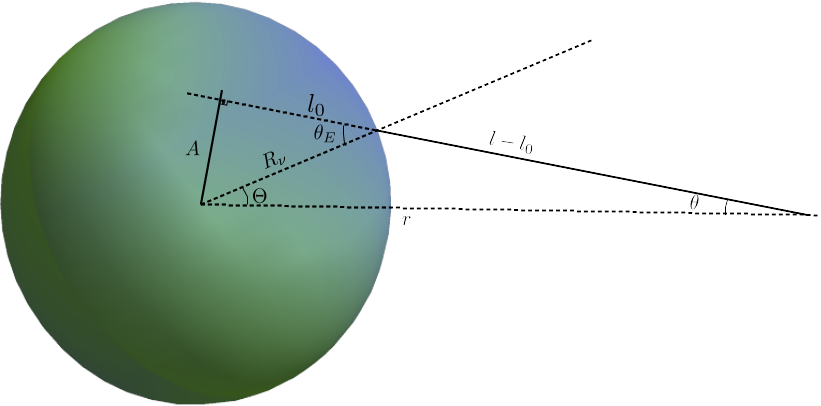
\includegraphics[width=0.7\textwidth]{figures/BulbModel.png}
    \caption[Ampul (Bulb) Modeli.]{Ampul (Bulb) Modeli. Bu şekil \cite{Duan:2006an} numaralı referanstan benzetilerek oluşturulmuştur.}
    \label{fig:BulbModel}
\end{figure}
Ampul modelinin temelde iki adet simetrisi vardır. Birincisi küresel simetri ikincisi ise radyal doğrultuda azimuthal simetridir. Azimuthal simetri, sistemin azimuthal açısından yani $ \varphi $ açısından bağımsız olduğu anlamına gelir. Buradaki $ \theta $ ve $ \varphi $ açıları küresel koordinatlardan gelen açılardır, $ \dd{\vec{r}} = \dd{r} \hat{r} + r\dd{\theta} \hat{\theta} + r\sin\theta\dd{\varphi} \hat{\varphi}  $.  Bu simetrileri, \eqref{eqn:NuKim_LiouvilleVonNeumann_multiAng} numaralı denkleme uygularsak
\begin{equation}
    i v_{r} \dv{r}\hat{\rho} = \comm{\hat{H}}{\hat{\rho}} \text{.}
\end{equation}
denklemi elde edilir. Burada $ v_{r} $, hız vektörünün radyal bileşenidir. Hareket denklemini hızdan bağımsız hale getirip saçılım açısı $ \theta $ ile alakalı hale getirmek için sinüs teoremi kullanılır. 
\begin{equation}
    \frac{\sin \theta}{R_{\nu}} = \frac{\sin \Theta}{l-l_{0}} \text{ .}
\end{equation}
Burada $ l= r\cos \theta $ ve $ l_{0} = R_{\nu} \cos \theta_{E} $ şeklindedir. $ R_{\nu} $ ise nötrinosferin yarıçapıdır ve nötrino evriminin başladığı uzaklıktır. Açıların geometri üzerindeki yerleri, \ref{fig:BulbModel} şeklinde gözükmektedir. $ \sin \theta_{E} $ ve $ \sin \theta $ arasındaki ilişki de aşağıdaki gibi yazılır.
\begin{align}
    \dfrac{\sin \theta}{R_{\nu}} = \dfrac{\sin \theta_{E}}{r} \text{ .}
\end{align}
Tüm bu ilişkiler bir araya getirildiğinde, sinüs teoremine benzer bir ifade elde edilir.
\begin{equation}
	\frac{\sin \theta}{R_{\nu}} = \frac{\sin \Theta}{l-l_{0}}=\dfrac{\sin \theta_{E}}{r} \label{eq:AngleRelations}
\end{equation}
Yukarıdaki bağıntı sayesinde iki bağımsız açı elde edebiliriz. 

Nötrinosferden seçilmiş $ r $ kadar uzaklığına kadar, sadece belli bir maksimum $ \theta_{E} $ yayılma açısıyla çıkan nötrino ulaşabilir. Örneğin seçilen bir $ P $ noktasına, proto-nötron yıldızının arka tarafından nötrino gelemez. Bu sınırlamayı $ \theta_{max} $ olarak gösterebiliriz. Açıkça ifadesi
\begin{equation}
    \theta_{max}=\arcsin \qty(\frac{R_{\nu}}{r})
\end{equation}
şeklinde olacaktır. Sonuç olarak rastgele bir $ r $ noktasına gelebilen nötrinoların ilgili açı karşılıklarını elde ettik.

Nötrinolar öz-kırılım etkilerini anlayabilmek için rastgele bir noktadaki, o noktaya $ P $ noktası diyelim, diferansiyel nötrino yoğunluğunu belirlememiz gerekir. $ \alpha $ çeşnisine sahip, $ r $ uzaklığında ve $ q $ enerjisine sahip nötrinoların diferansiyel sayı yoğunluğu aşağıdaki gibi yazılır.
\begin{equation} \label{eq:DiffNumberDensity1}
    \dd{n_{\nu_{\alpha}}}(\vec{q}) = j_{\nu_{\alpha}}(q) \cos \theta_{E}  ~~ \frac{1}{(l-l_{0})^{2}} ~~ R^{2}_{\nu} \dd(\cos \Theta) \dd \Phi \text{ .}
\end{equation}
Burada $j_{\nu_{\alpha}}(q)$, $ \alpha $ çeşnisine sahip olan $ q $ enerjili nötrino sayı akısı (flux), $ (l-l_{0})^{-2} $ geometrik genişlemeden (dilation) gelen terim ve $ R^{2}_{\nu} \dd(\cos \Theta) \dd \Phi $ terimi diferansiyel hacim kısmıdır. Burada  $j_{\nu_{\alpha}}(q)$ terimi sadece ileri saçılan nötrinoları kapsar. Şimdi elde ettiğimiz geometrik bağıntıları kullanarak \eqref{eq:DiffNumberDensity1} numaralı denklemi sadeleştirebiliriz.
\begin{align}\label{eq:DiffNumberDensity2}
    \nonumber\dd{n_{\nu_{\alpha}}}(\vec{q}) &= j_{\nu_{\alpha}}(q) \cos \theta_{E}  ~~ \frac{1}{(l-l_{0})^{2}} ~~ R^{2}_{\nu} \dd(\cos \Theta) \dd \Phi\\
	\nonumber &= j_{\nu_{\alpha}}(q) \frac{R^{2}_{\nu}}{(l-l_{0})^{2}} ~~  \cos \theta_{E} ~~ \dfrac{(l-l_{0}) \sin \theta}{R_{\nu}} ~~\dfrac{(l-l_{0}) \dd \theta}{R_{\nu} \cos \theta_{E}} ~~\dd \Phi\\
	 &= j_{\nu_{\alpha}}(q) \dd (\cos \theta) \dd \phi  \text{ .}
\end{align}
Burada $ \cos \theta_{E} R_{\nu} \dd \Theta = (l-l_{0}) \dd \theta $ bağıntısı kullanılmıştır. Ayrıca geometri bize $ \dd \Phi = \dd \phi $ bağıntısını verir.

Elde edilen \eqref{eq:DiffNumberDensity2} numaralı bağıntı yardımıyla $ r $ yarıçaplı bir küre yüzeyinden geçen toplam nötrino sayısı şöyle yazılır.
\begin{align}
    \nonumber \text{Toplam } \nu_{\alpha} \text{ sayısı }&= 4\pi r^{2} \int \cos \theta \dd n_{\nu_{\alpha}} \\
    &= 4\pi^{2}R_{\nu}^{2}j_{\nu_{\alpha}}(q) \text{ .}
\end{align}

Toplam $ \alpha $ çeşnisine sahip olan nötrino sayısı başka bir şekilde de ifade edilebilir.
\begin{equation}\label{eq:NumberOfNeutrinos}
    4\pi R^{2}_{\nu}\int^{1}_{0}2\pi j_{\nu_{\alpha}} \cos \theta_{E} \dd (\cos \theta_{R}) = 4\pi^{2}R_{\nu}^{2}j_{\nu_{\alpha}}(q) \text{ .}
\end{equation}
$ r $ noktasındaki nötrino akısı da aşağıdaki gibi tanımlanır.
\begin{align}\label{eq:FluxofNeutrinos}
    4\pi R^{2}_{\nu}\int^{1}_{0}2\pi j_{\nu_{\alpha}} \cos \theta_{E} \dd (\cos \theta_{R}) = \dfrac{L_{\nu_{\alpha}}}{\expval{E_{\nu_{\alpha}}}} f_{\nu_{\alpha}} \text{ .}
\end{align}
Burada $ L_{\nu_{\alpha}} $ nötrino parlaklığı (luminosity), $ \expval{E_{\nu_{\alpha}}} $ ortalama nötrino enerjisi ve $f_{\nu_{\alpha}}  $ normalize edilmiş enerji dağılımıdır. \eqref{eq:NumberOfNeutrinos} ve \eqref{eq:FluxofNeutrinos} numaralı denklemler birleştirildiğinde, nötrino akısı elde edilir.
\begin{equation}
    j_{\nu_{\alpha}}=\dfrac{L_{\nu_{\alpha}}}{4\pi^{2}R^{2}_{\nu} \expval{E_{\nu_{\alpha}}}}f_{\nu_{\alpha}} \text{ .}
\end{equation}
Nötrinolar proto-nötron yıldızı içerisinde termalize olmuşlardır. Bundan dolayı başlangıçtaki enerji dağılımları ve sıcaklıkları güzel tanımlıdır. Nötrinoların spin $ 1/2 $ parçacıklar yani fermiyon olduğu dikkate alındığında başlangıçtaki dağılımları Fermi-Dirac dağılımıdır.
\begin{align}
	f_{\nu_{\alpha}}(q) \equiv \dfrac{1}{F_{2}(\eta_{\nu_{\alpha}})}\dfrac{1}{T^{3}_{\nu_{\alpha}}}\dfrac{q^{2}}{\exp \qty(q/T_{\nu_{\alpha}} - \eta_{\nu_{\alpha}})+1} \text{ .}
\end{align}
Burada $ \eta_{\nu_{\alpha}} $ dejenerelik parametresidir. $ F_{2}(\eta_{\nu_{\alpha}}) $ terimi ise Fermi-Dirac integrali ve $ T_{\nu_{\alpha}} $, $ \alpha $ çeşnisine sahip nötrinoların sıcaklığıdır. Bu çalışmada dejenerelik parametresi sıfır alınacaktır. Nötrinolar ultra-göreli parçacıklar olduğu için momentum büyüklüğü $ q $ yerine enerji $ E $ yazılabilir.

Nötrinoların proto-nötron yıldızı içerisinde termalize olma aşamalarında farklılıklar olabilir \cite{Keil:2002in}. Yüksek enerjili nötrinolar biraz daha fazla etkileştikleri için nötrinosferin daha dış yani soğuk katmanlarında ayrışırlar. Yani her ne kadar nötrinolar termal dengeye gelmiştir, belli bir sıcaklığı vardır desek de aslında yüksek enerjili nötrinolar bundan biraz daha soğuk, düşük enerjili nötrinolar biraz daha sıcaktır. Bunun sonucu olarak spektrum Fermi-Dirac olmaktan bir miktar sapar. Bu farklılığı parametrize ederek Fermi-Dirac dağılımı \emph{sıskalaştırılır} (pinched). Sıska dağılım aşağıdaki gibi yazılır.
\begin{equation}
    f_{\nu_{\alpha}}(E) \equiv \dfrac{\beta^{\beta}}{\Gamma (\beta)} \dfrac{E^{\beta-1}}{\expval{E_{\nu_{\alpha}}}^{\beta}} \exp (\beta E/E_{\nu_{\alpha}}) \text{ .}
\end{equation}
Burada $ \beta $ spektral parametre ve $ \Gamma (\beta) $ ise Euler Gamma fonksiyonudur. Bu parametreler model bağımlıdır. Bu çalışmada kullanılmasa da nötrino öz-kırılım çalışmalarında sıska dağılım oldukça popülerdir, çünkü öz-kırılımlar altındaki çeşni evrimi spektruma çok bağlıdır. Genelde $ \beta=3 $ parametresi seçilse de $ \beta=4 $ seçilen çalışmalar da mevcuttur \cite{Dasgupta:2010cd}. Son olarak ortalama nötrino enerjisi ile sıcaklık arasında aşağıdaki gibi bir bağlantı vardır.
\begin{align}
    \nonumber \expval{E_{\nu_{\alpha}}} = & \dfrac{\int^{\infty}_{0} E f_{\nu_{\alpha}}(E)\dd{E} }{\int^{\infty}_{0} f_{\nu_{\alpha}}(E)\dd{E} } \\
    \nonumber & = \frac{F_{3}(0)}{F_{2}(0)}T_{\nu_{\alpha}} \\
    \approx & ~3.1516 ~ T_{\nu_{\alpha}}
\end{align}
Burada Fermi-Dirac integrali, $ F_{n}(0) \equiv \int \dd{x} \frac{x^{n}}{e^{x}+1} $ şeklinde tanımlanmıştır.

İlerleme hız vektörüne bağlı olarak yazılan \eqref{eqn:NuKim_LiouvilleVonNeumann_multiAng} numaralı hareket denklemi nötrino saçılma açısı $ \theta $ cinsinden tekrar yazılabilir \cite{Sigl:1993ctk,Cardall:2007zw}.
\begin{equation}
    i \cos \theta \dv{r} \hat{\rho}(E,r,\theta) = \comm{\hat{H}(E,r,\theta)}{\hat{\rho}(E,r,\theta)} \text{.}
\end{equation}
Bu denklem kullanılarak çeşitli sayısal modeller elde edilebilir. Bu tip yaklaşıklığa \emph{çok-açı yaklaşıklığı} (multi-angel approximation) adı denir. Yoğunluk operatörü saçılma açısından bağımsız olarak alınırsa, hareket denkleminin serbestlik derecesi bir derece azalır. Bu durumda saçılma açısı $ \theta= 0 $ şeklinde alınır. Bahsedilen bu yaklaşıklığa da \emph{tek-açı yaklaşıklığı} (single-angle approximation) adı verilir. Tek-açı yaklaşıklığında hareket denklemi \eqref{eqn:NuKim_LiouvilleVonNeumann} numaralı denkleme indirgenir.

Tek-açı yaklaşıklığı ile çok-açı yaklaşıklığı arasında çözüm farkları olacaktır. Özellikle nötrino öz-kırılım dikkate alındığında çok-açı yaklaşıklığı kollektif nötrino salınımlarında gecikmeye sebep olacaktır \cite{Duan:2010bf}. Çok-açı yaklaşıklığının etkileri proto-nötron yıldızından daha uzak noktalarda kollektif salınımın başlaması dışında fazla etkisi bulunmamaktadır. Diğer taraftan geç başlayan kollektif salınımlar $ \nu p $ çekirdek sentezlenmesi gibi süpernova içerisindeki nükleer dinamikleri de etkileyecektir \cite{Sasaki:2017jry}.

Çok-açı yaklaşıklığı parametre uzayını, saçılma açı modu (saçılma açı aralığının kaç parça olacağı) kadar katlayacaktır. Hali hazırda bulunan diferansiyel denklem hem doğrusal değildir hem de çiftlenmiştir. Bu duruma ek olarak öz-kırılım Hamiltonyen'i, proto-nötron yıldızına yakın noktalarda çok yüksek değerdedir ve yüksek frekanslı çeşni salınımına sebep olur. Runge–Kutta–Fehlberg gibi dışsal (extrinsic) veya LSODA gibi hem içsel (intrinsic) hem dışsal diferansiyel denklem çözme algoritmaları bilgisayar kaynaklarını oldukça harcar. Bu sebeplerden dolayı bu çalışmada tek-açı yaklaşıklığı kullanılmıştır.

Nötrino öz-kırılım Hamiltonyen operatörü \eqref{eqn:Hamil_nunuOperator}, çok-açı ve tek-açı yaklaşıklığına göre değişir. Çok-açı yaklaşıklığında nötrino öz-kırılım Hamiltonyen'i aşağıdaki gibi olur.
\begin{align}
    \nonumber \hat{H}_{\nu\nu}(r)=& \sqrt{2}G_{F} \sum_{\alpha,\beta = e,x} \int \dd{\dd{n_{\nu_{\alpha}}}} (1-cos \theta) \qty[\qty[\rho_{\alpha\beta}(E,r,\theta)-\rho_{\bar{\alpha}\bar{\beta}}(E,r,\theta)]] \\
    &\times \qty(\dyad{\nu_{\alpha}}{\nu_{\beta}}-\dyad{\nu_{\bar{\alpha}}}{\nu_{\bar{\beta}}}) \text{ .}
\end{align}
Saçılım açısını $ \theta=0 $ alıp nötrino sayı yoğunluğunu, $ \dd{n_{\nu_{\alpha}}} $, da yerine koyduğumuzda, tek-açı yaklaşıklığına sahip nötrino öz-kırılım Hamiltonyen'i elde edilir \cite{Duan:2006an}.
\begin{align}
    \nonumber \hat{H}_{\nu\nu}(r)=& \sum_{\alpha,\beta = e,x} \int \dd{E} \qty[\rho_{\alpha\beta}(E,r)f_{\nu_{\alpha}}(E) \frac{L_{\nu_{\alpha}}}{\expval{E_{\nu_{\alpha}}}} -\rho_{\bar{\alpha}\bar{\beta}}(E,r) f_{\nu_{\bar{\alpha}}}(E) \frac{L_{\nu_{\bar{\alpha}}}}{\expval{E_{\nu_{\bar{\alpha}}}}} ] \\
    &\times \sqrt{2}G_{F} D_{T}(r)\qty(\dyad{\nu_{\alpha}}{\nu_{\beta}}-\dyad{\nu_{\bar{\alpha}}}{\nu_{\bar{\beta}}}) \text{ .}
\end{align}
Burada $ D_{T}(r) $ katsayısı
\begin{equation}
    D_{T}(r) = \frac{1}{2} \qty[1- \sqrt{1- \qty(\frac{R_{\nu}}{r})^{2}}]^{2}
\end{equation}
şeklinde verilir. Tek açı yaklaşıklığı altında nötrino öz-kırılımın etkisi, $ 1/r^{2} $ gibi azalmaktadır. Bu nedenle nötrino öz-kırılım Hamiltonyen'i proto-nötron yıldızının yakınlarında baskın olur.

\section{OYUNCAK MODELLER}\label{sec:OyuncakModel}
\paragraph{}
Oyuncak modelleri oluştururken madde profilini yani ortamdaki baryonun konumla nasıl değiştiğini analitik olarak bildiğimizi varsayıyoruz. Bunun sayesinde, \ref{sec:evrim} numaralı bölümde verilen birçok analitik öngörü kullanılabilir olmaktadır. Oyuncak modeller olarak adlandırdığımız ve bu başlık altındaki tüm simülasyonlarda baryon profili, aksi belirtilmedikçe aşağıdaki gibi olacaktır.
\begin{equation}
    n_{b}(r) = 10^{6} \exp(-\frac{r}{r_{mat}}) \text{ [g/cm$^3$] .}
\end{equation}
Burada santimetre küp başına kaç gram baryon düştüğü verilmiştir. $ r_{mat} $ olarak verilen ifade ise baryon yoğunluğunun eksponansiyel olarak nasıl düşeceğini belirten katsayıdır ve birimi [km] cinsindendir. Oyuncak modeller için kullandığımız simülasyonlarda bu değer $ r_{mat}=200 $ km olarak alınacaktır. Analitik baryon profili ve kullanılan değerler rastgele seçilmemiştir. Bu değerler, süpernova simülasyonunun $ t=5 $ s'deki baryon profiline fit edilmiş değerleridir.

Oyuncak model simülasyonları da kendi içerisinde 9'a ayrılacaktır. İki ana simülasyonun 9'ar alt simülasyonlara bölünmesinin sebebi nötrino-manyetik etkileşimlerinde başlangıç koşullarının küçük değişiminin sonuçlara olan etkisine bakılmasıdır. Başlangıç koşullarındaki küçük değişimler ortalama yoğunluk operatörünün \emph{ortalama} değerini neredeyse etkilemeyecektir. Sayısal sonuçların değişimi ise \eqref{eqn:rhoBar_hata} denkleminde verilen \emph{hata} oranından düşük bir oranda değişmesi beklenmektedir, çünkü sistemde yapılan küçük değişikliklerin evrime olan etkisi, evrimin fazlarından kaynaklanan terimler kadar kendisini gösterecektir. \eqref{eqn:rhoBar_hata} numaralı denklemde maksimum ve minimum fazlar dikkate alındığı için sayısal sonuçların hata barının içerisinde kalması beklenmektedir. 

Sayısal sonuçlar ile analitik sonuçları karşılaştırmadan önce iki "ana" simülasyonun ortak başlangıç parametrelerini aşağıdaki tabloda verebiliriz. Dış madde yoğunluk profili ve dış manyetik alan profili \ref{tab:simulasyonlar} numaralı tabloda verilmiştir. Bu tabloda verilen değerler \cite{ParticleDataGroup:2018ovx} numaralı kaynaktan alınmıştır.
\begin{table}[hbt!]
    \centering
    \begin{tabular}{|c|c|}
        \hline Çeşni Sayısı & $4$ \\
        \hline Hiyerarşi & Ters \\
        \hline Boşluk Karışım Açısı [Rad]& $0.14$ \\
        \hline CP Fazı [Rad] & $ 0 $ \\
        \hline Kütle Kare Farkı [MeV$^{2}$] & $2.4 \times 10^{-15}$ \\
        \hline Nötrino Manyetik Momenti [$ \mu_{B} $] & $ 5\times10^{-16} $ \\
        \hline Nötrino Enerji Aralığı [MeV] & $1$-$50$  \\
        \hline Son uzaklık [km] & $4000$ \\
        \hline Nötrino İstatistiksel Dağılımı & Sadece Elektron, kutu dağılımı  \\
        \hline
    \end{tabular}
    \caption[Oyuncak Modellerin Ortak Başlangıç Koşulları.]{\label{tab:oyuncakModOrtakBasKos}Oyuncak Modellerin Ortak Başlangıç Koşulları. theta014expNbB adlı modelde normal hiyerarşi ve sadece elektron antinötrino kutu dağılımı da kullanılmıştır.}
\end{table}

Oyuncak model olarak yapılan iki simülasyonun birbirinden tek farkı karışım açısıdır. \emph{theta0expNbB} adlı simülasyonda boşluk karışım açısı sıfırdır. \emph{theta014expNbB} adlı simülasyonda ise boşluk karışım açısı $ 0.14 $ olarak alınmıştır. Bu, $\theta_{13} $ boşluk salınım açısı değeridir \cite{ParticleDataGroup:2018ovx}. Bu ve \ref{tab:oyuncakModOrtakBasKos} numaralı tabloda verilen değerler kullanılarak oyuncak model oluşturulmuş ve simülasyonlar yapılmıştır.

Oyuncak modellerin simülasyon sonuçlarına geçmeden önce her bir oyuncak modelin $ 9 $ alt simülasyonu hakkında bilgi vereceğiz. Tüm başlangıç koşullar, \ref{tab:simulasyonlar} ve \ref{tab:oyuncakModOrtakBasKos} numaralı tabloda verilmiştir. Bu koşullardan, simülasyonun başlangıç uzaklığı $ R $ ve dış manyetik alanın azalma parametresi $ r_{Mag} $ üzerinde küçük değişiklikler yapılacaktır. Bu değişiklikler \ref{tab:oyuncakModel9BasKosul} numaralı tabloda verilmiştir.

\begin{table}[hbt!]
    \centering
    \begin{tabular}{|c|c|c|}
        \hline $ R=49.90 $, $ r_{Mag}=50.1 $& $ R=49.90 $, $ r_{Mag}=50.05 $ & $ R= 49.90$, $ r_{Mag}=50 $\\
        \hline $ R=49.95 $, $ r_{Mag}=50.1 $& $ R=49.95 $, $ r_{Mag}=50.05 $ & $ R= 49.95$, $ r_{Mag}=50 $\\
        \hline $ R=50.00 $, $ r_{Mag}=50.1 $& $ R= 50.00$, $ r_{Mag}=50.05 $ & $ R= 50.00$, $ r_{Mag}=50 $\\
        \hline
    \end{tabular}
    \caption[Oyuncak Modellere Ait 9 Alt Simülasyonun Başlangıç Koşulları.]{\label{tab:oyuncakModel9BasKosul}Oyuncak Modellere Ait 9 Alt Simülasyonun Başlangıç Koşulları. Buradaki tüm değerler km birimindedir.}
\end{table}

\textbf{theta0expNbB} adlı simülasyonun analitik ve sayısal sonuçları, karşılaştırılmalı olarak \ref{fig:theta0expNbB_9x9_10MeV} numaralı şekilde verilmiştir.

\begin{figure}[hbt!]
    \centering
    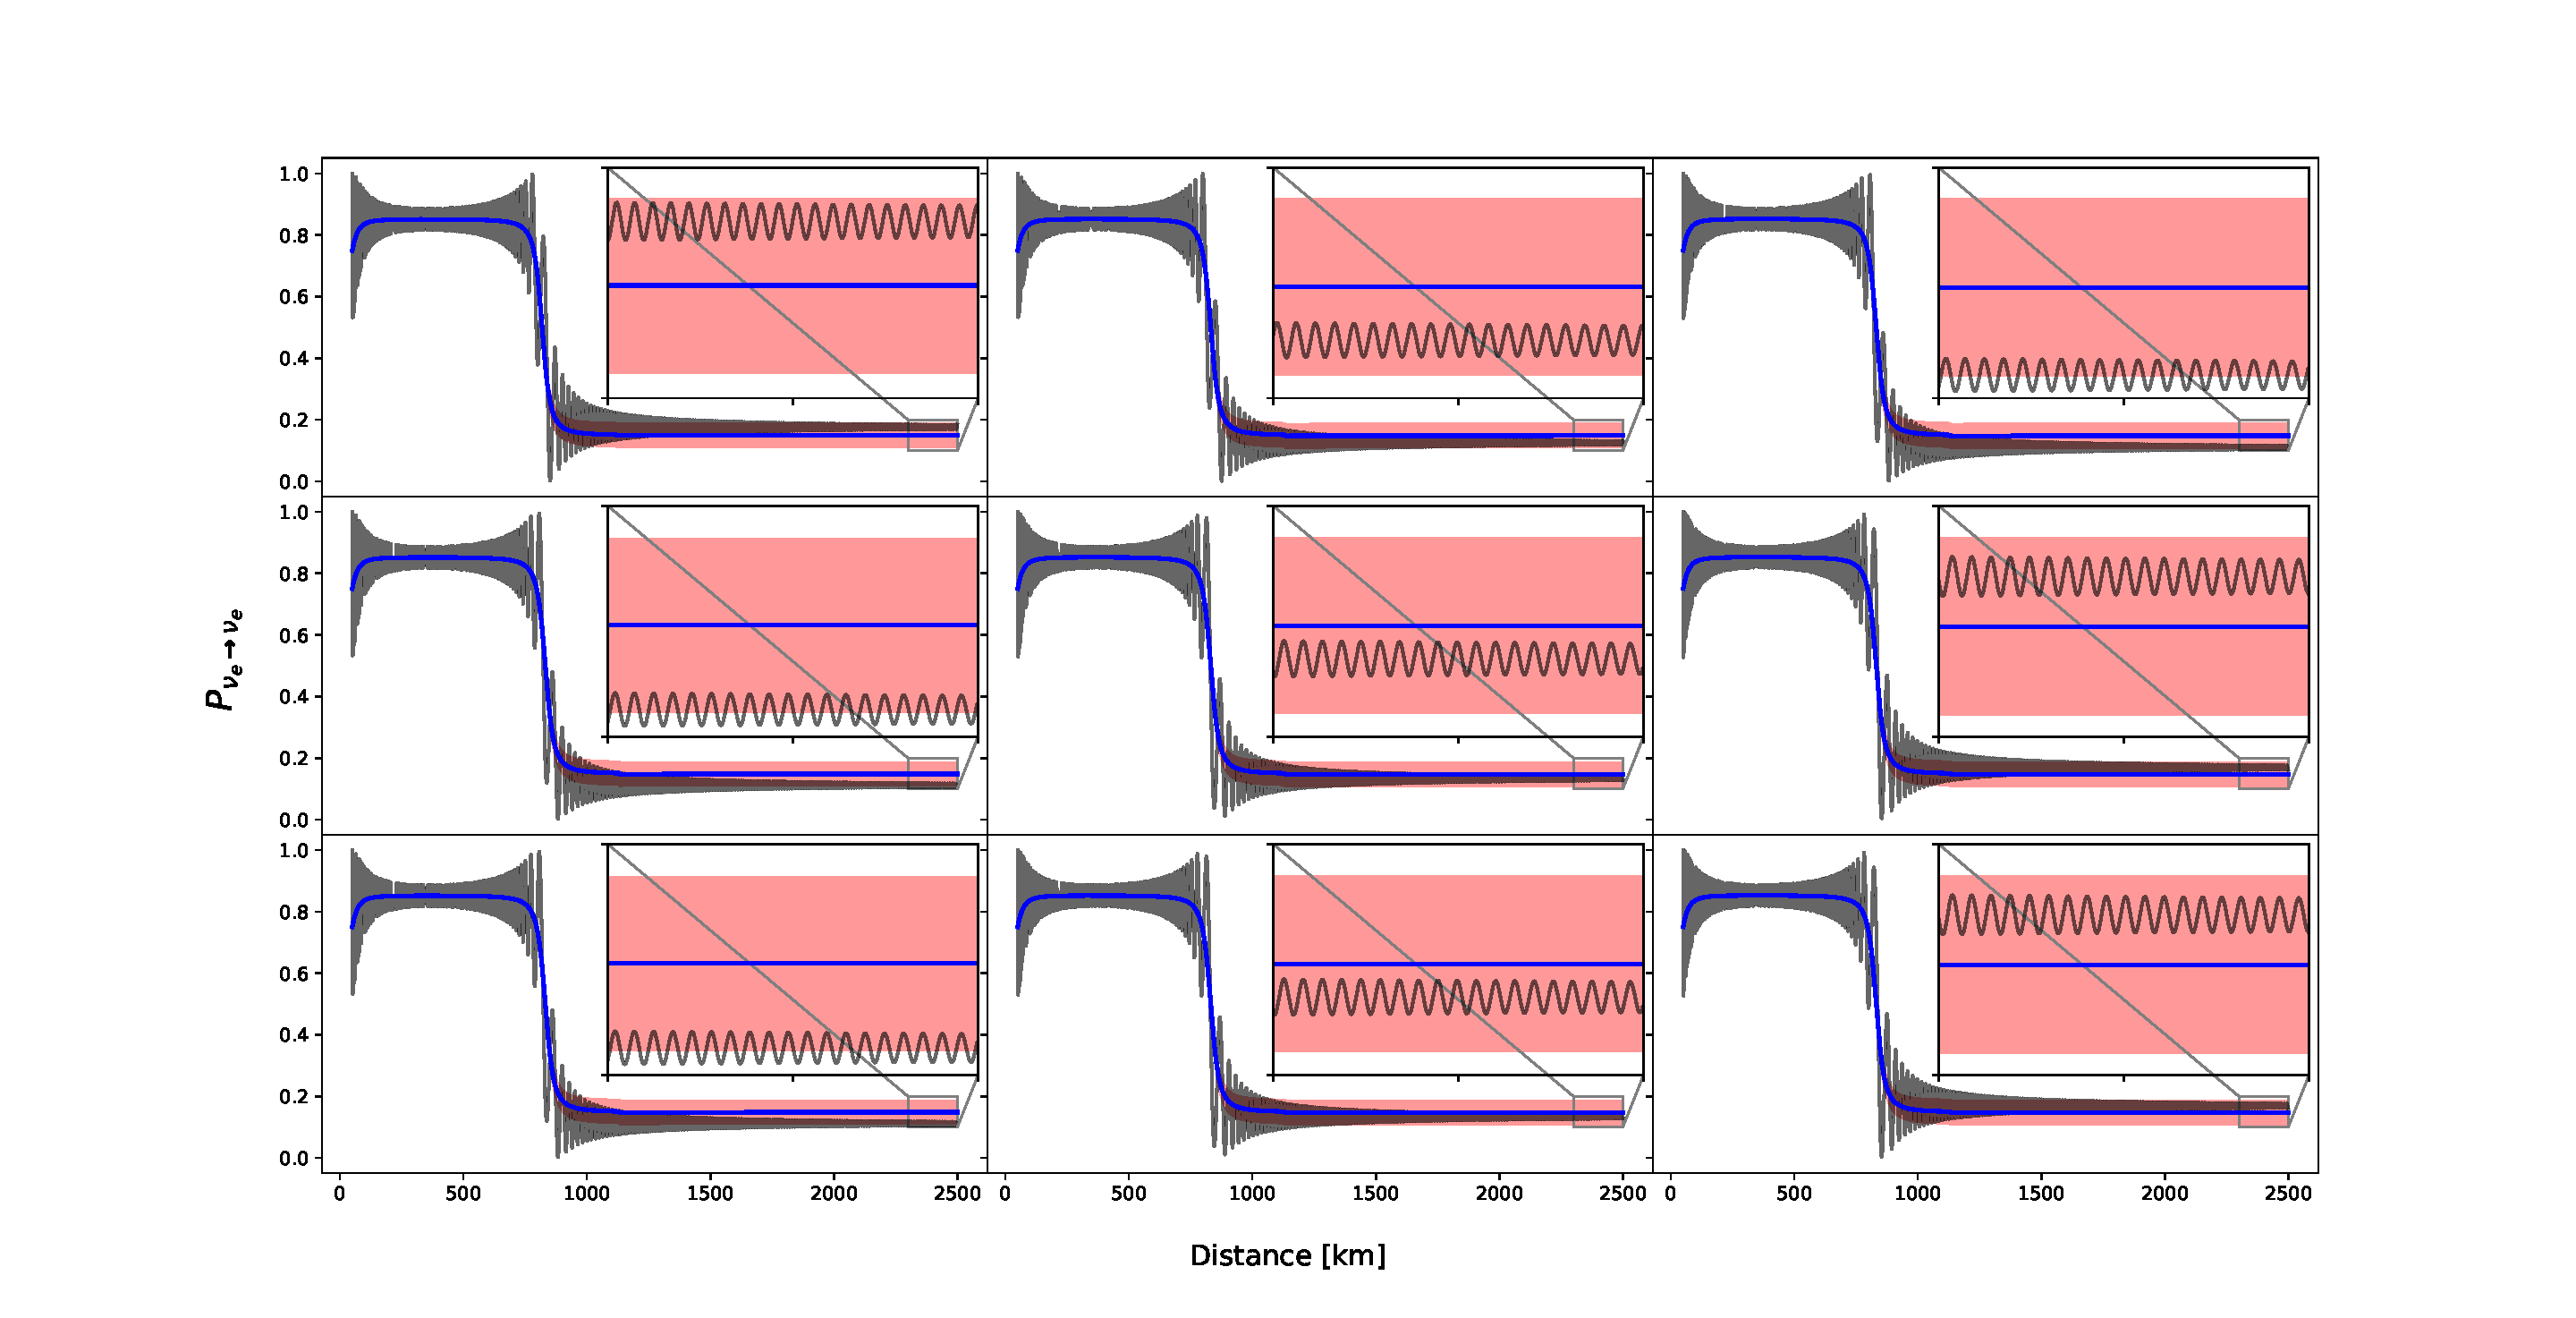
\includegraphics[width=1\textwidth]{figures/theta0expNbB_9x9_10MeV.pdf}
    \caption[theta0expNbB Modelinin, 9 Alt Simülasyonun, $ 10 $ MeV İçin Uzaklığa Karşılık Yaşama Olasılıkları.]{theta0expNbB Modelinin, 9 Alt Simülasyonun, $ 10 $ MeV İçin Uzaklığa Karşılık Yaşama Olasılıkları. Siyah çizgiler simülasyonların sayısal sonuçları, mavi çizgiler analitik öngörü sonuçlarını ve kırmızı aralıklar ise analitik öngörüden sapmaları, yani hatayı göstermektedir. Alt simülasyonların başlangıç koşullarındaki farklar, \ref{tab:oyuncakModel9BasKosul} numaralı tabloda verilmiştir ve sıralama da bu tablodaki gibidir.}
    \label{fig:theta0expNbB_9x9_10MeV}
\end{figure}

Boşluk karışım açısı sıfır olduğunda MSW rezonansı gözükmemesi beklenmektedir. \ref{fig:theta0expNbB_9x9_10MeV} numaralı grafikten de görüldüğü gibi sadece SFP rezonansı meydana gelmektedir.$ 10 $ MeV enerjili nötrinoların SFP rezonansı yaklaşık $830$ km'de meydana gelmiştir ve theta0expNbB simülasyonları için SFP rezonansının LZ geçiş olasılıkları $ 0.003 $ mertebesindedir. Bu geçiş olasılığını veren adyabatisite parametresi ise $ 0.9 $'dur.

Analitik olarak elde ettiğimiz bağıntılar \eqref{eqn:rhoBar_ort} ve \eqref{eqn:rhoBar_hata} numaralı formüller ile verilmiştir. Bu formüllerin, \ref{fig:theta0expNbB_9x9_10MeV} numaralı şekildeki hangi terimlere denk geldiğini açıklayabiliriz. Analitik olarak elde edilen ortalama yoğunluk matris elemanları grafikte mavi çizgi olarak gösterilmiştir. Mavi çizgiler, siyah olan sayısal çözümlerin ortalaması olarak ilerlemektedir. SFP rezonansından sonra da sayısal çözümler ortalama etrafında salınmaya devam etmektedir. Sayısal çözümlerin salınım genlikleri düştüğünde ise ortalama teriminden sapmalar açığa çıkmaktadır. Bu sapmanın tek sebebi rezonansın adyabatik olmamasıdır. Adyabatik olmayan geçişlerde ise fazlar kendisini gösterir. Faz ile orantılı olan analitik sonuçlar ise \eqref{eqn:rhoBar_hata} numaralı bağıntıda verilmiştir. Bu bağıntıda fazların maksimum ve minimum olduğu terim \ref{fig:theta0expNbB_9x9_10MeV} numaralı şekilde kırmızı alan olarak işaretlenmiştir. Yaptığımız çalışmada sayısal sonuçlar ile theta0expNbB adlı model için analitik sonuçlarla tam olarak uyum göstermektedir. Sadece $ R=49.9 $ km, $ r_{mag}=50.1 $ km için olan sonuçlar, \ref{fig:theta0expNbB__R49_9_rmag50_1_10MeV} numaralı grafikte daha yakından gösterilmiştir.

\begin{figure}[hbt!]
    \centering
    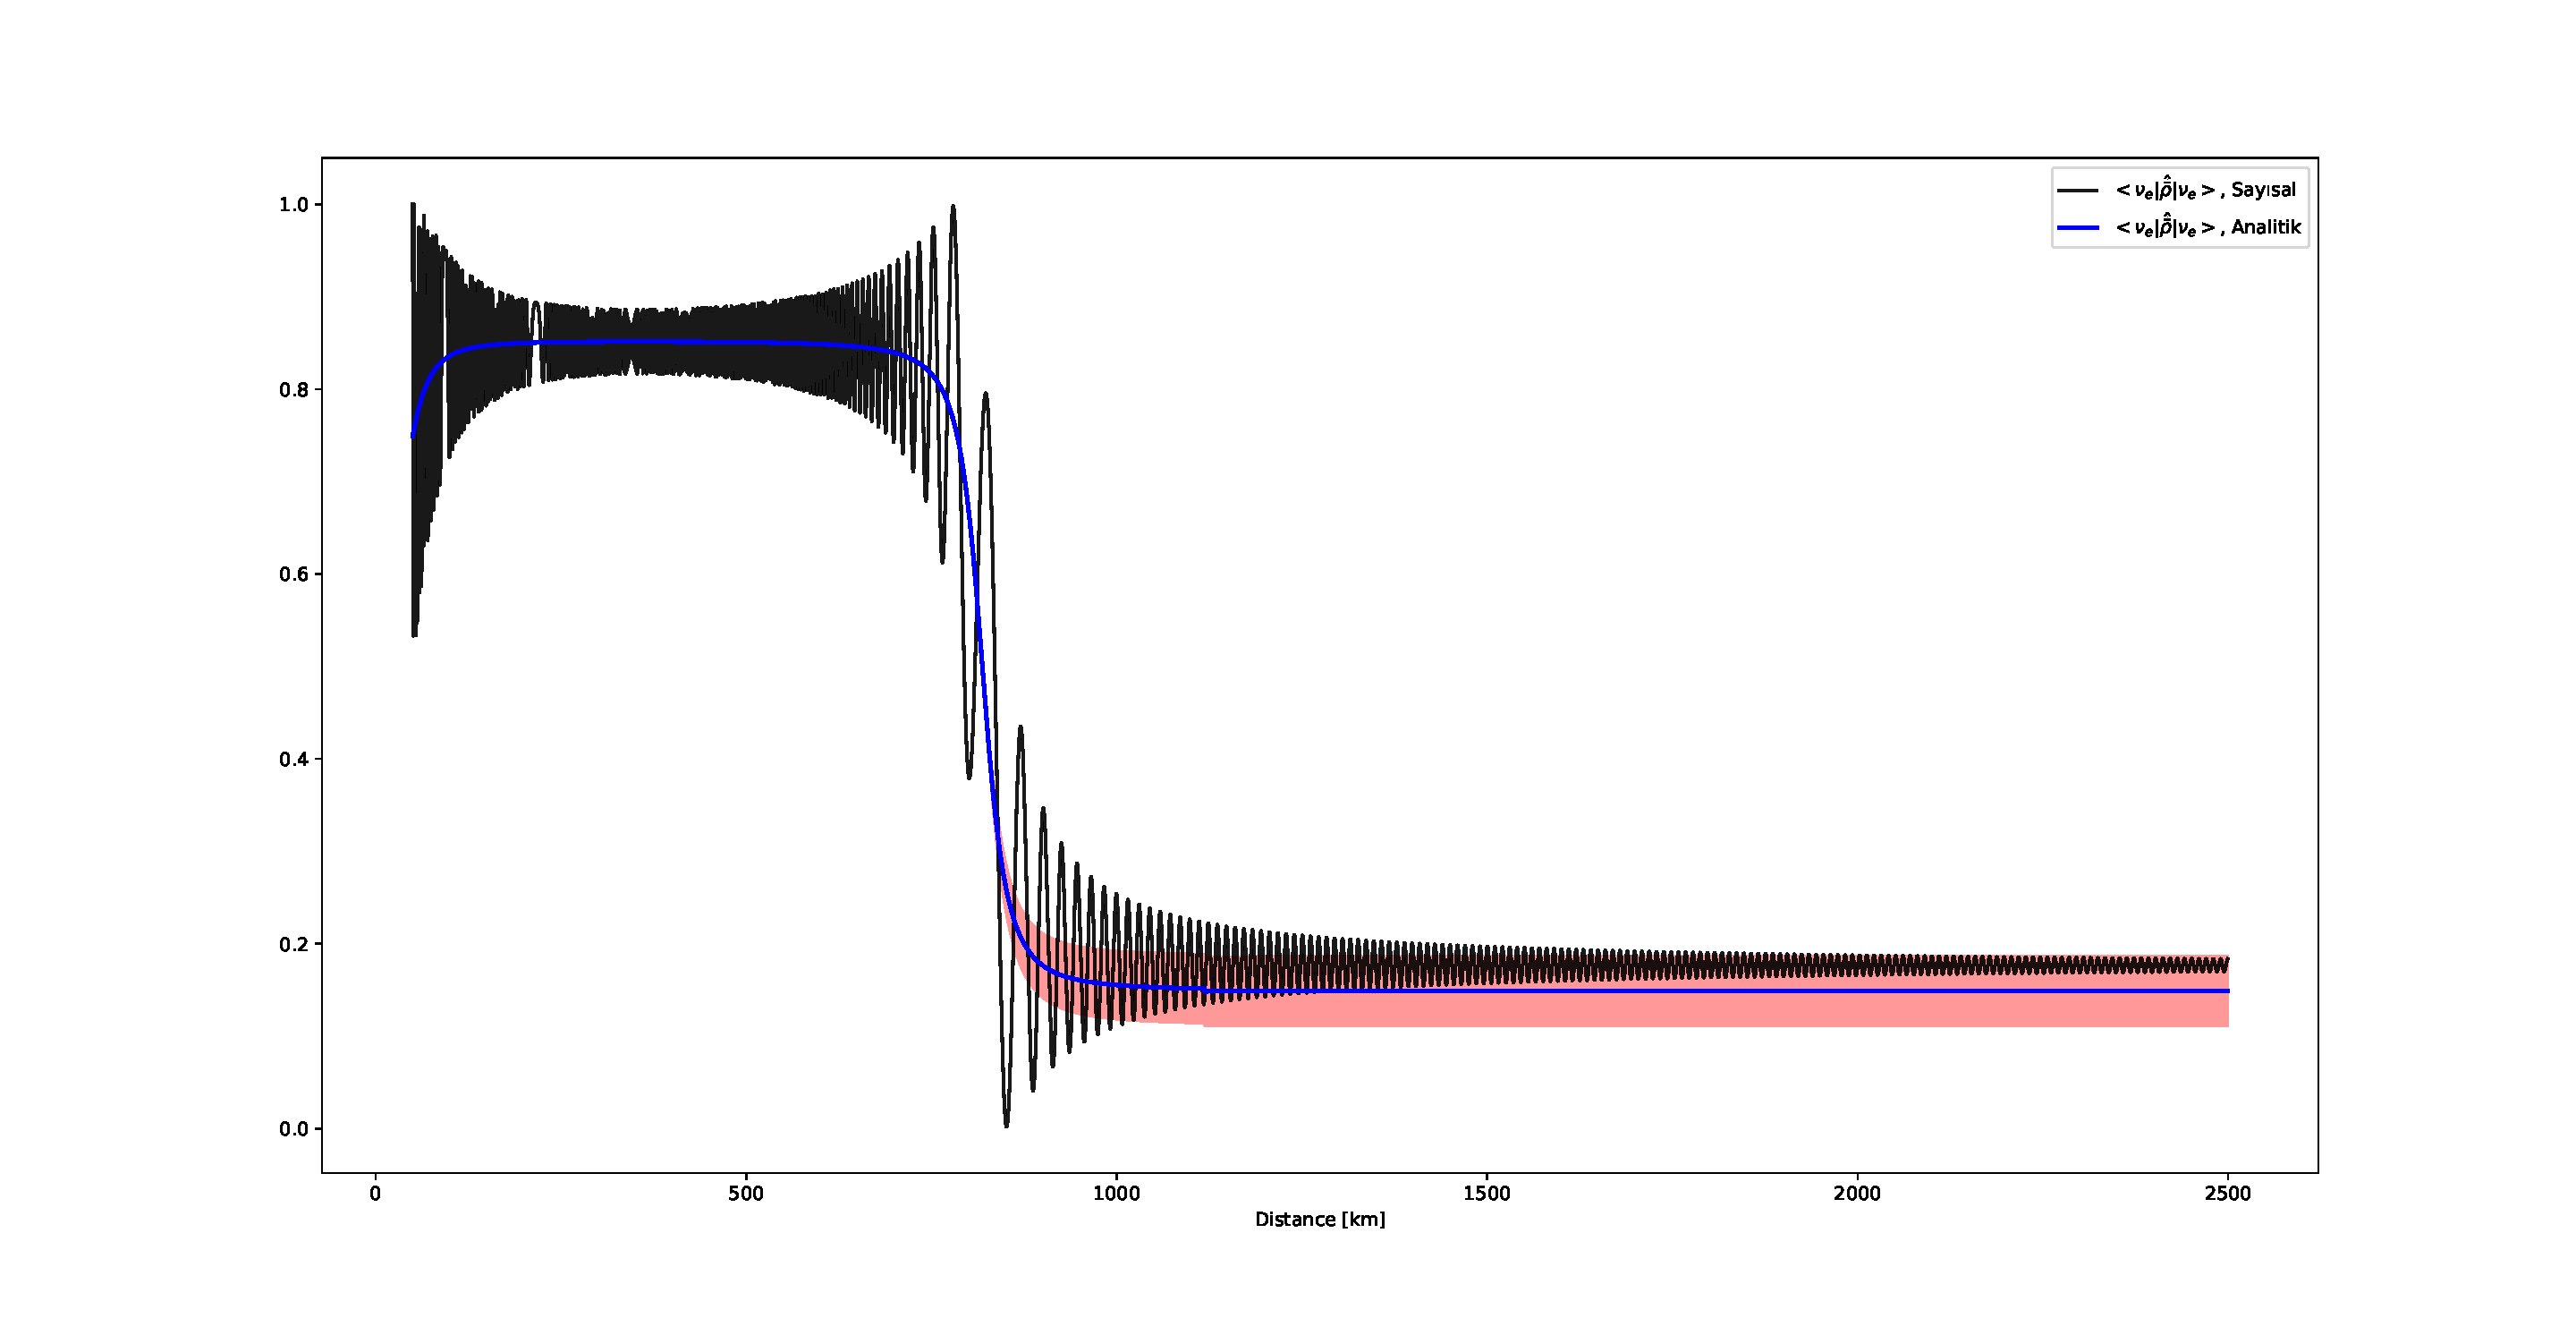
\includegraphics[width=1\textwidth]{figures/theta0expNbB_R49_9_rmag50_1_10MeV.pdf}
    \caption[theta0expNbB Modeli, $ R=49.9 $ km, $ r_{mat}=50.1 $ km simülasyonu ve $ 10 $ MeV İçin Uzaklığa Karşılık Yaşama Olasılıkları]{theta0expNbB Modeli, $ R=49.9 $ km, $ r_{mat}=50.1 $ km simülasyonu ve $ 10 $ MeV İçin Yaşama Olasılıkları}
    \label{fig:theta0expNbB__R49_9_rmag50_1_10MeV}
\end{figure}

theta0expNbB modeli için 9 farklı alt simülasyon yapmamızın sebebi şudur; başlangıç koşullarındaki küçük değişiklikler, fazlardan kaynaklanan sonsuzdaki sayısal çözümlerde küçük değişiklikler meydana getirir. Bu küçük değişikler altında analitik ve sayısal çözümlerin uyumlu olup olmadığına bakılmıştır. Boşluk karışım açısının sıfır olduğu bu simülasyonlar, öngördüğümüz analitik hata aralığı dahilinde doğru sonuçlar vermiştir. 

Elde edilen bu sonuçlar her enerji için geçerlidir. \ref{fig:theta0expNbB_energySpec_theta0_averaged} numaralı grafikte son yaşama olasılıklarının enerjiye göre dağılımı verilmiştir. Bu grafikte mavi çizgiler her enerjideki ortalamanın simülasyon sonundaki değerini göstermektedir. Siyah noktalar ise 9 farklı simülasyonun en son ortalama sayısal değeridir. Yukarıda verilen ve $10$ MeV için geçerli olduğunu gösterdiğimiz analitik ve sayısal sonuç karşılaştırmaları her enerji için geçerlidir. Yani her bir enerji için analitik ve sayısal çözümler tutarlıdır. Düşük enerjide hata aralığının küçülmesi veya yok olmasının sebebi, bu enerjiler için evrimin adyabatik olmasıdır. Adyabatik evrimde $ P_{SFP} $ terimi sıfırdır. Bundan dolayı \eqref{eqn:rhoBar_hata} terimi de sıfır olarak gelecektir. Hata olarak tabir ettiğimiz kırmızı bölge de düşük enerjilerde olmayacaktır.

\begin{figure}[hbt!]
    \centering
    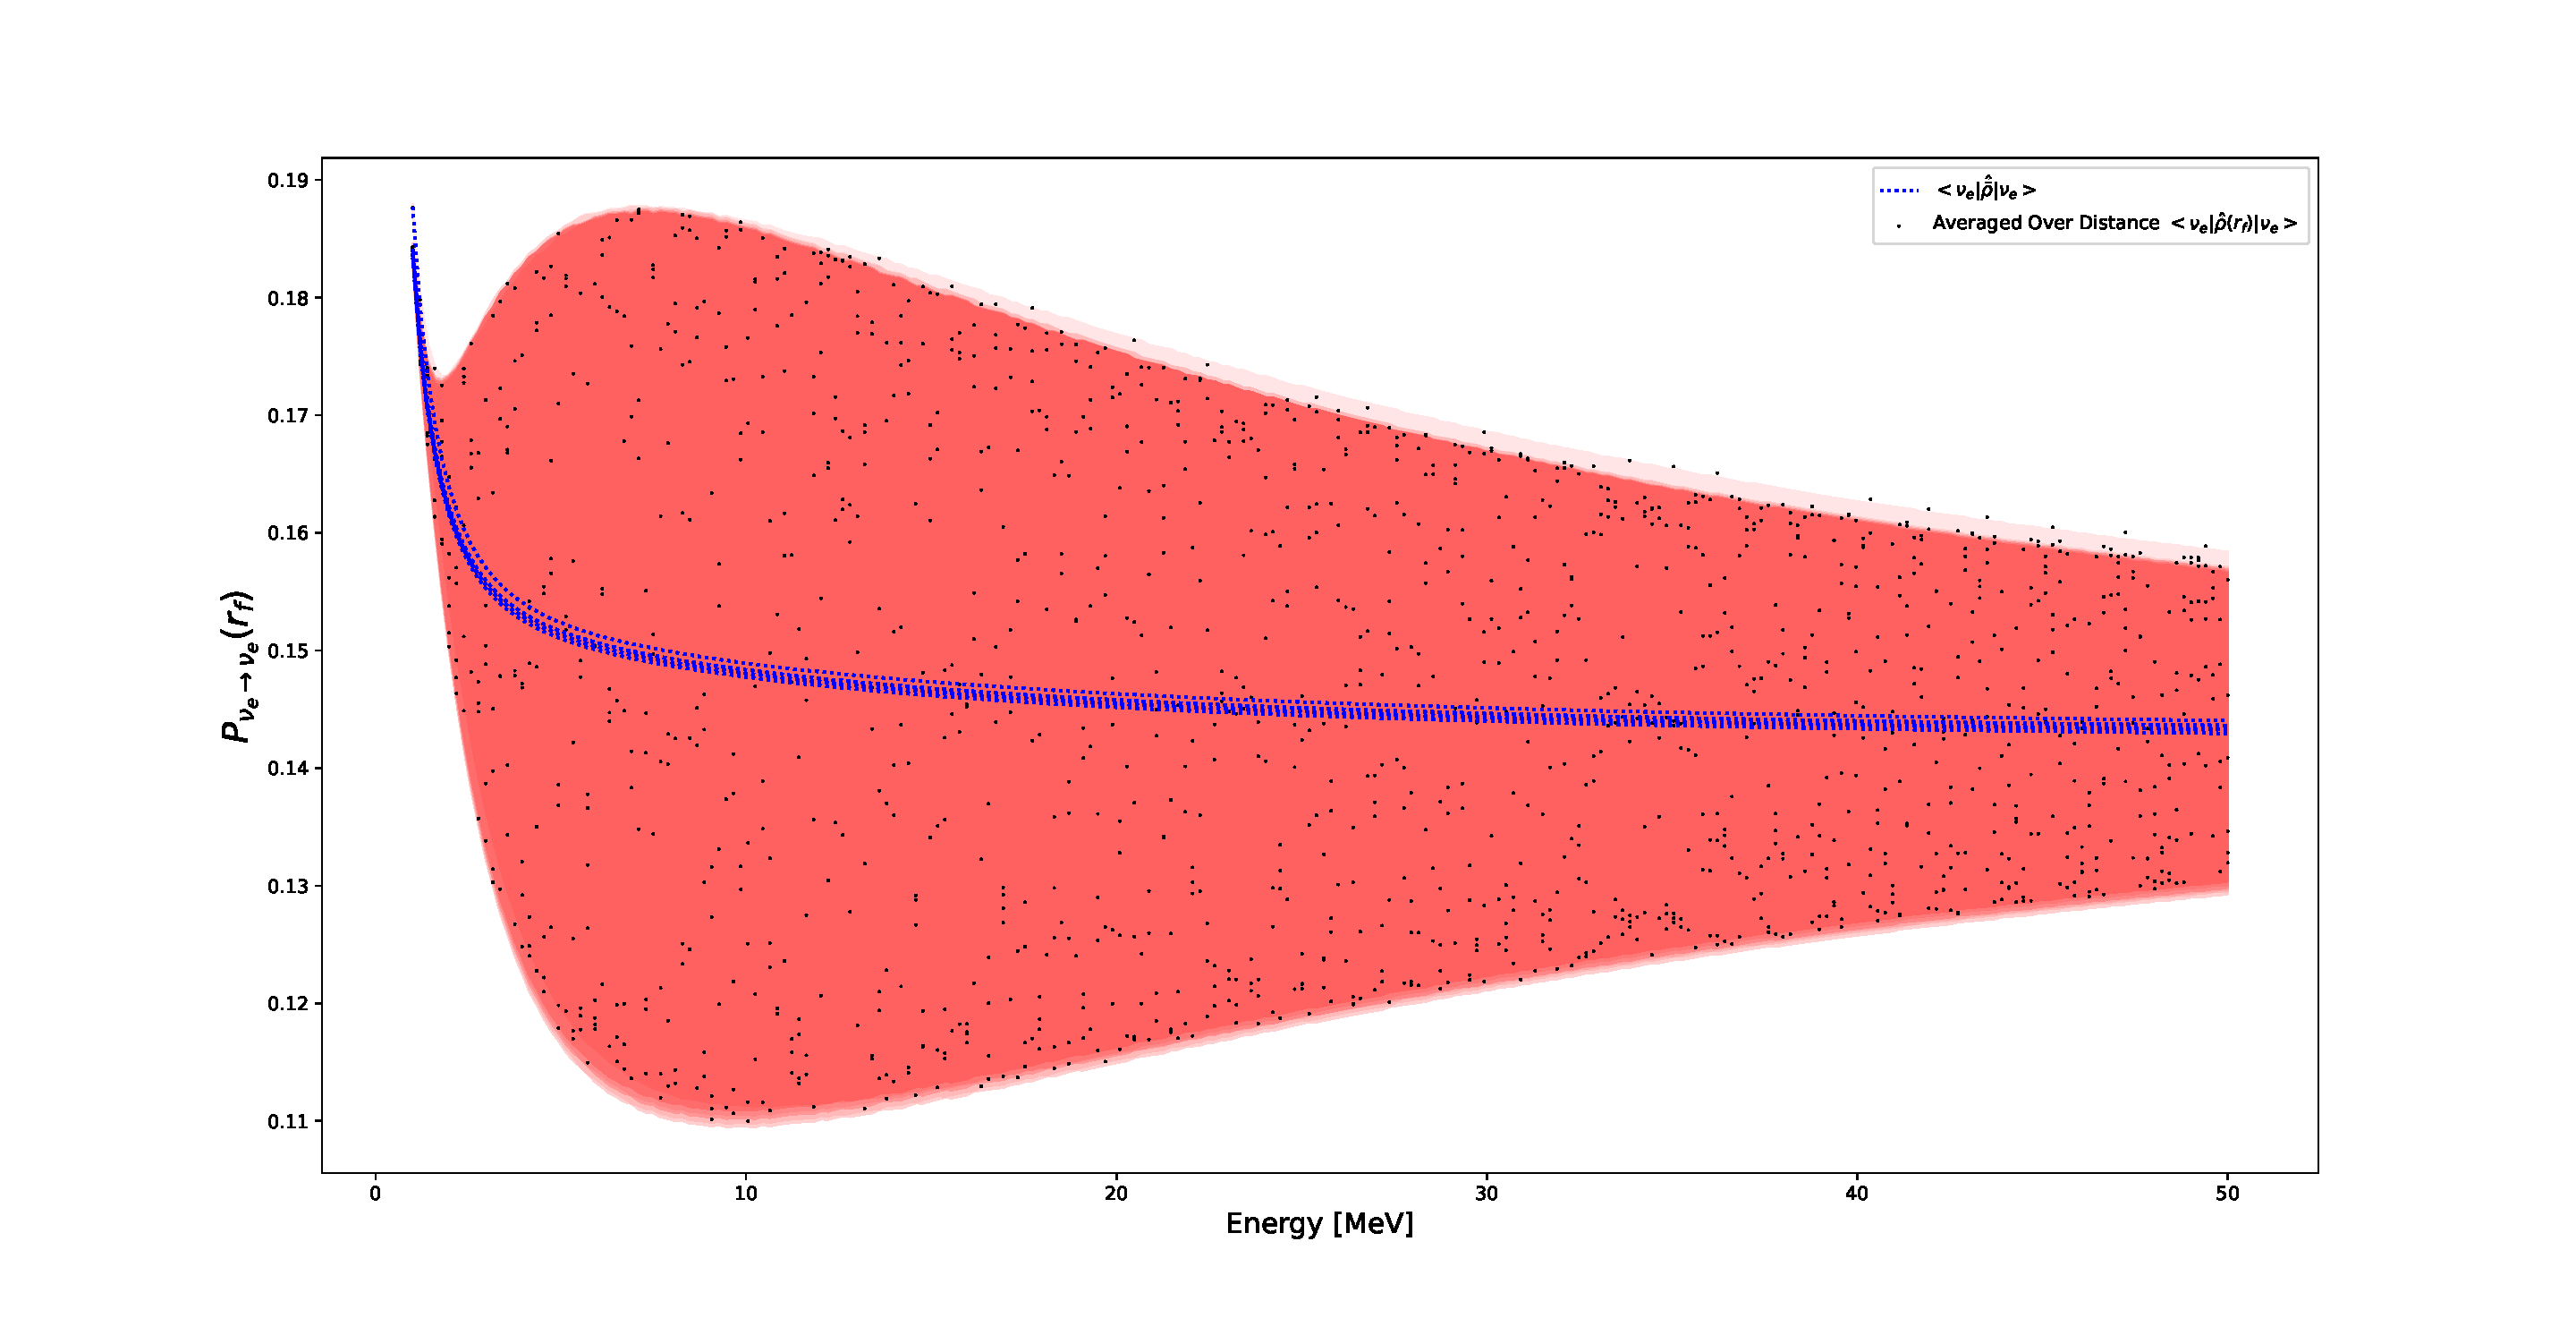
\includegraphics[width=\textwidth]{figures/theta0expNbB_energySpec_theta0_averaged.pdf}
    \caption[theta0expNbB Modeli, 9 simülasyonun Enerjiye Karşılık Yaşama Olasılıkları]{theta0expNbB Modeli, 9 simülasyonun Enerjiye Karşılık Yaşama Olasılıkları. Her siyah nokta, sayısal sonuçların son birkaç kilometredeki ortalamasıdır.}
    \label{fig:theta0expNbB_energySpec_theta0_averaged}
\end{figure}

Fazların çeşni evrimine olan etkisi de \ref{fig:theta0expNbB_energySpec_theta0_averaged} numaralı grafikten gözükmektedir. Her enerji için yapılan 9 simülasyon sonucunda sayısal sonuçlar belli bir noktada olmayıp bir aralık arasında "rastgele" dağılmaktadır. LZ geçiş olasılığından kaynaklanan hata aralığı, $ 10 $ MeV civarında en yüksek değere ulaşmıştır. Bu sonuç, Dünya'dan yapılacak olan nötrino algıç (detect) deneylerinden SN modelleri oluşturulmasında önemli yer tutar.

\textbf{theta014expNbB} adlı simülasyonun analitik ve sayısal sonuçları, karşılaştırılmalı olarak \ref{fig:theta014expNbB_9x9_10MeV} numaralı şekilde verilmiştir.

\begin{figure}[hbt!]
    \centering
    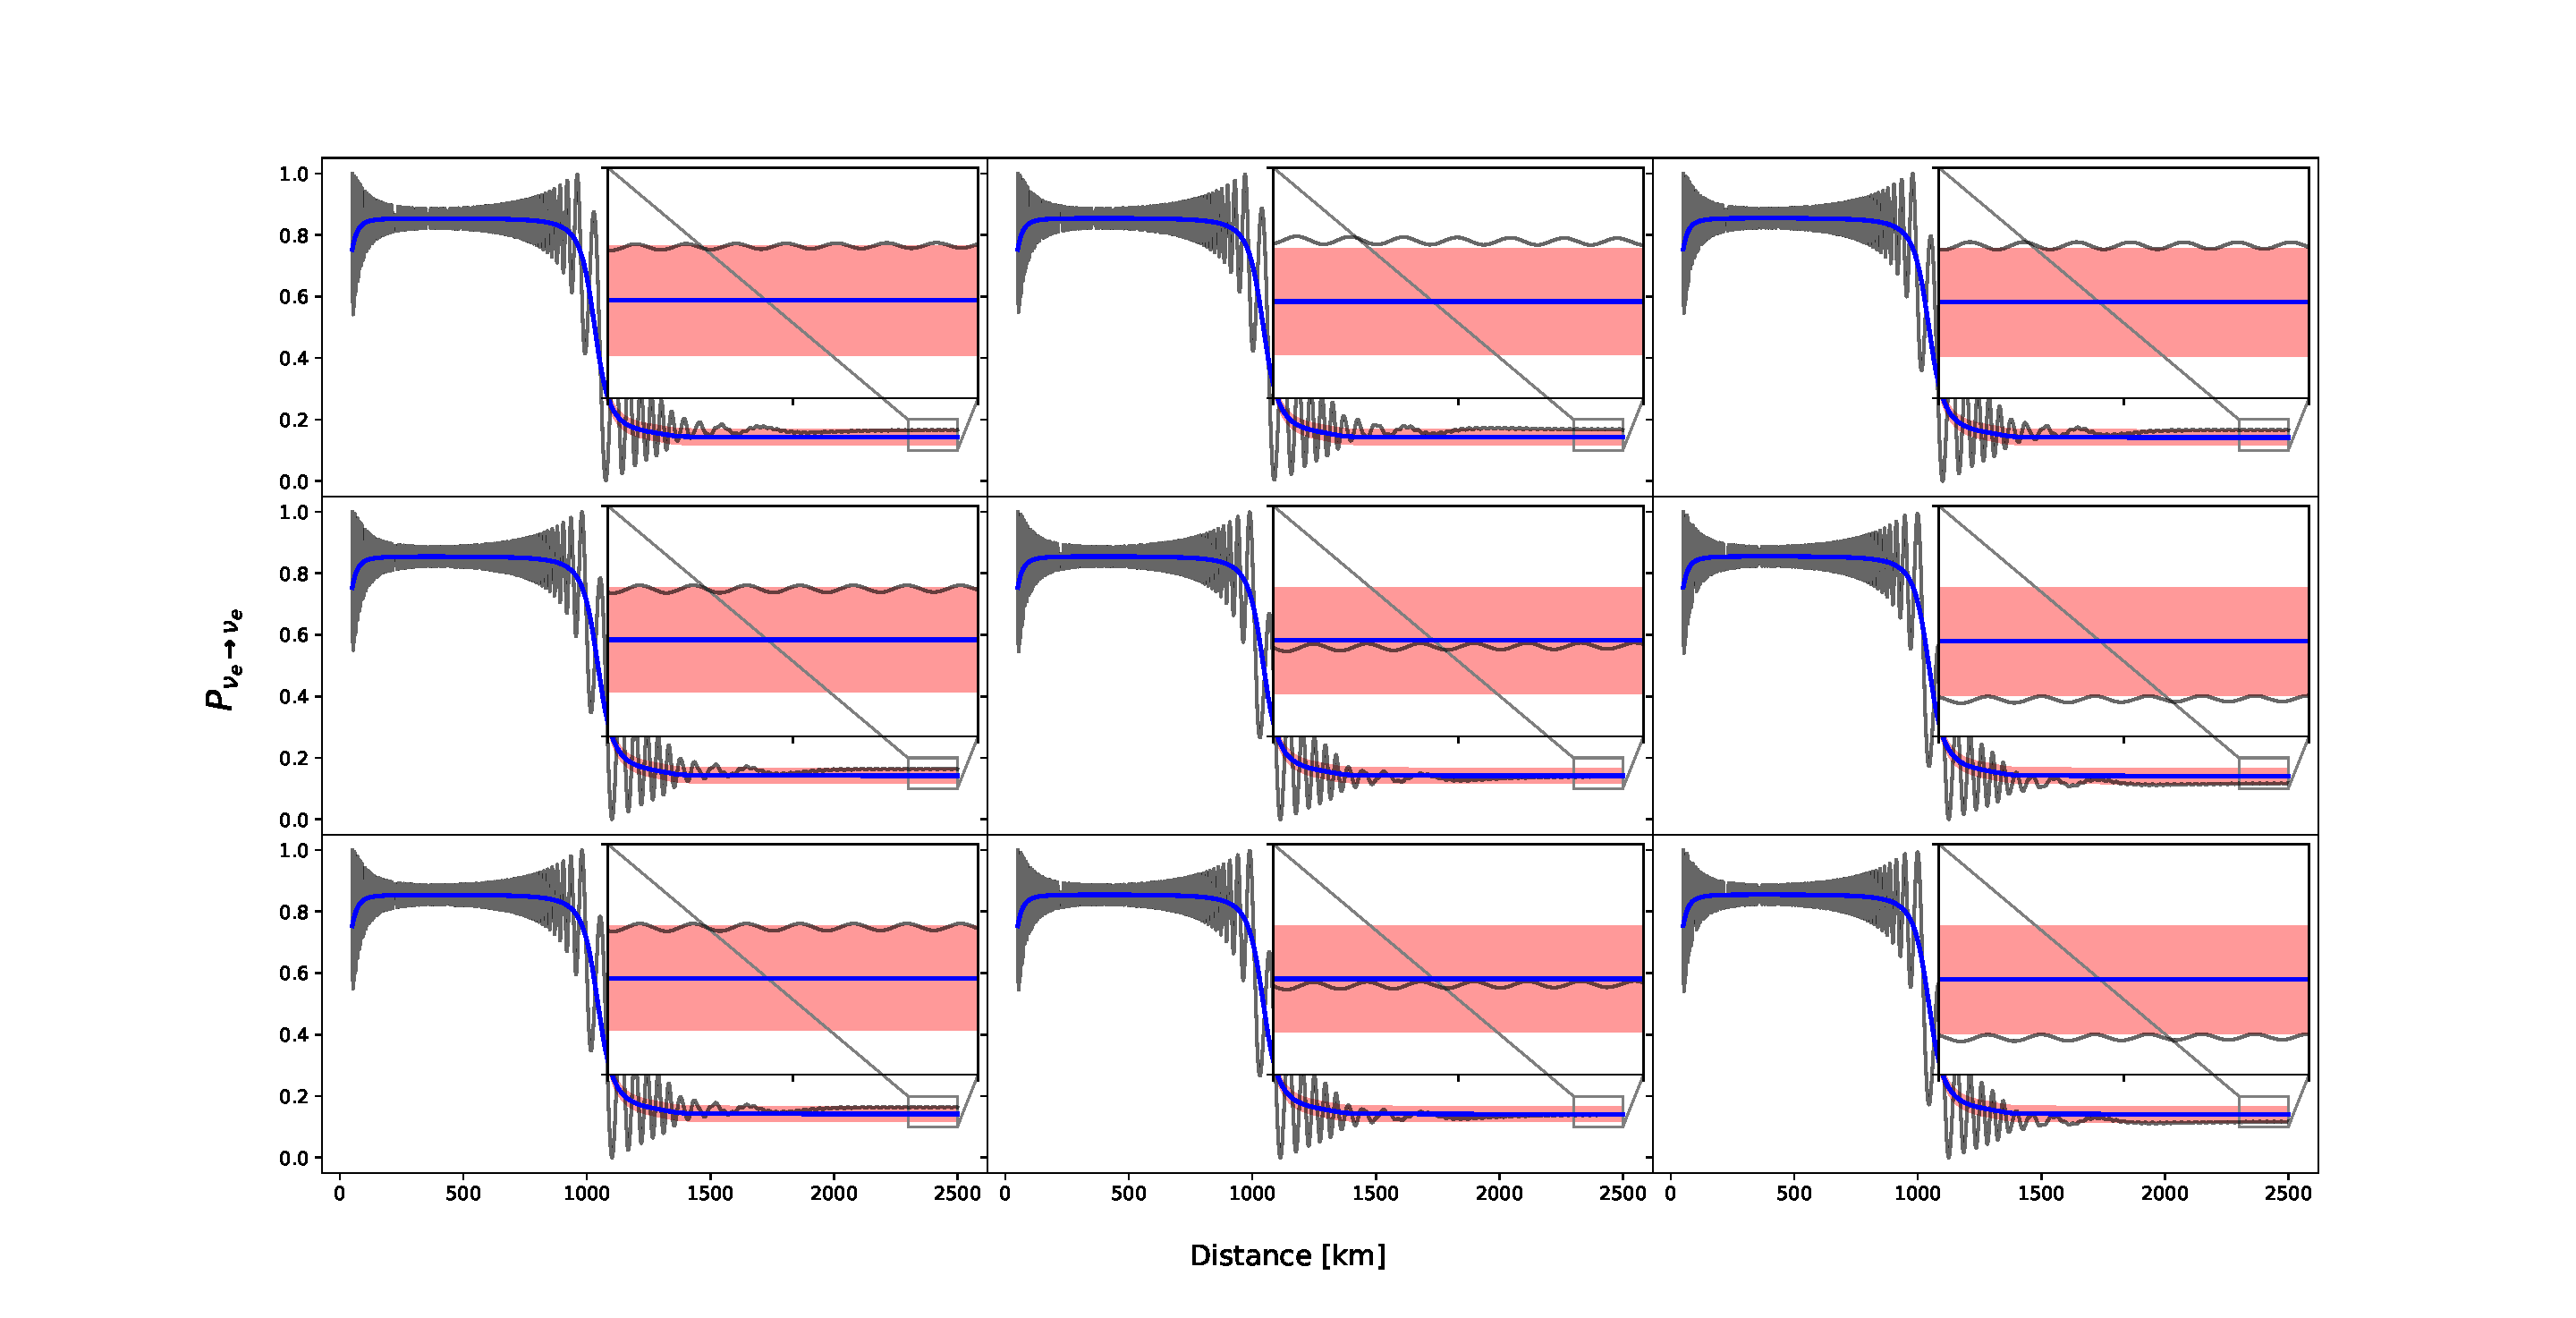
\includegraphics[width=\textwidth]{figures/theta014expNbB_9x9_10MeV.pdf}
    \caption[theta014expNbB Modelinin, 9 Alt Simülasyonun, $ 10 $ MeV İçin Uzaklığa Karşılık Yaşama Olasılıkları]{theta014expNbB Modelinin, 9 Alt Simülasyonun, $ 10 $ MeV İçin Uzaklığa Karşılık Yaşama Olasılıkları. Siyah çizgiler simülasyonların sayısal sonuçları, mavi çizgiler analitik öngörü sonuçlarını ve kırmızı aralıklar ise analitik öngörüden sapmaları, yani hata aralığını göstermektedir. $ 10 $ MeV enerjisi için, ($ R=49.90 $, $ r_{Mag}=50.05 $), ($ R= 49.90$, $ r_{Mag}=50 $), ($ R= 49.95$, $ r_{Mag}=50 $) ve ($ R= 50.00$, $ r_{Mag}=50 $) başlangıç koşullarına sahip olan simülasyon sonuçları analitik öngörü ile uyuşmamaktadır.}
    \label{fig:theta014expNbB_9x9_10MeV}
\end{figure}

Karışım açısının sıfır olmadığı durumda SFP rezonansına ek olarak MSW rezonansı da gerçekleşecektir. \ref{fig:theta014expNbB_9x9_10MeV} numaralı şekil $ 10 $ MeV enerjili nötrinolar için çizilmiş olup SFP rezonansı yaklaşık $840$ km'de meydana gelmiştir. MSW rezonansı ise $ 1270 $ km civarında meydana gelmektedir. theta014expNbB simülasyonları için SFP LZ geçiş olasılıkları $ 0.003 $ mertebesinde ve MSW geçiş olasılıkları $ 10^{-14} $ mertebesindedir. Bu geçiş olasılığını veren adyabatisite parametresi ise SFP için $ 0.9 $, MSW için $ 4.8 $ mertebesindedir.

theta0expNbB modelinden farklı olarak theta014expNbB modelinde, analitik olarak elde ettiğimiz bağıntılar \eqref{eqn:rhoBar_ort} \eqref{eqn:rhoBar_hata} numaralı formüller ile bazı sayısal çözümlerin uyuşmadığı görülmektedir. Bu MSW ve SFP rezonanslarının iki ayrı $ 2\times2 $ sistem olarak ele alınmasından kaynaklanan bir hatadır diyebiliriz. Öncelikle bu durumun $ 10 $ MeV ile sınırlı olmadığını, tüm enerjilerde bir miktar uyumsuzluk olduğunu söylemek gerekir. \ref{fig:theta014expNbB_energySpec_theta0_averaged} numaralı grafikten de açıkça görüldüğü gibi siyah nokta ile gösterilen sayısal çözümler kırmızı ile verilen hata aralığın dışına çıkmıştır. Hatta yüksek enerjili nötrinolarda fark büyümektedir.

\begin{figure}[hbt!]
    \centering
    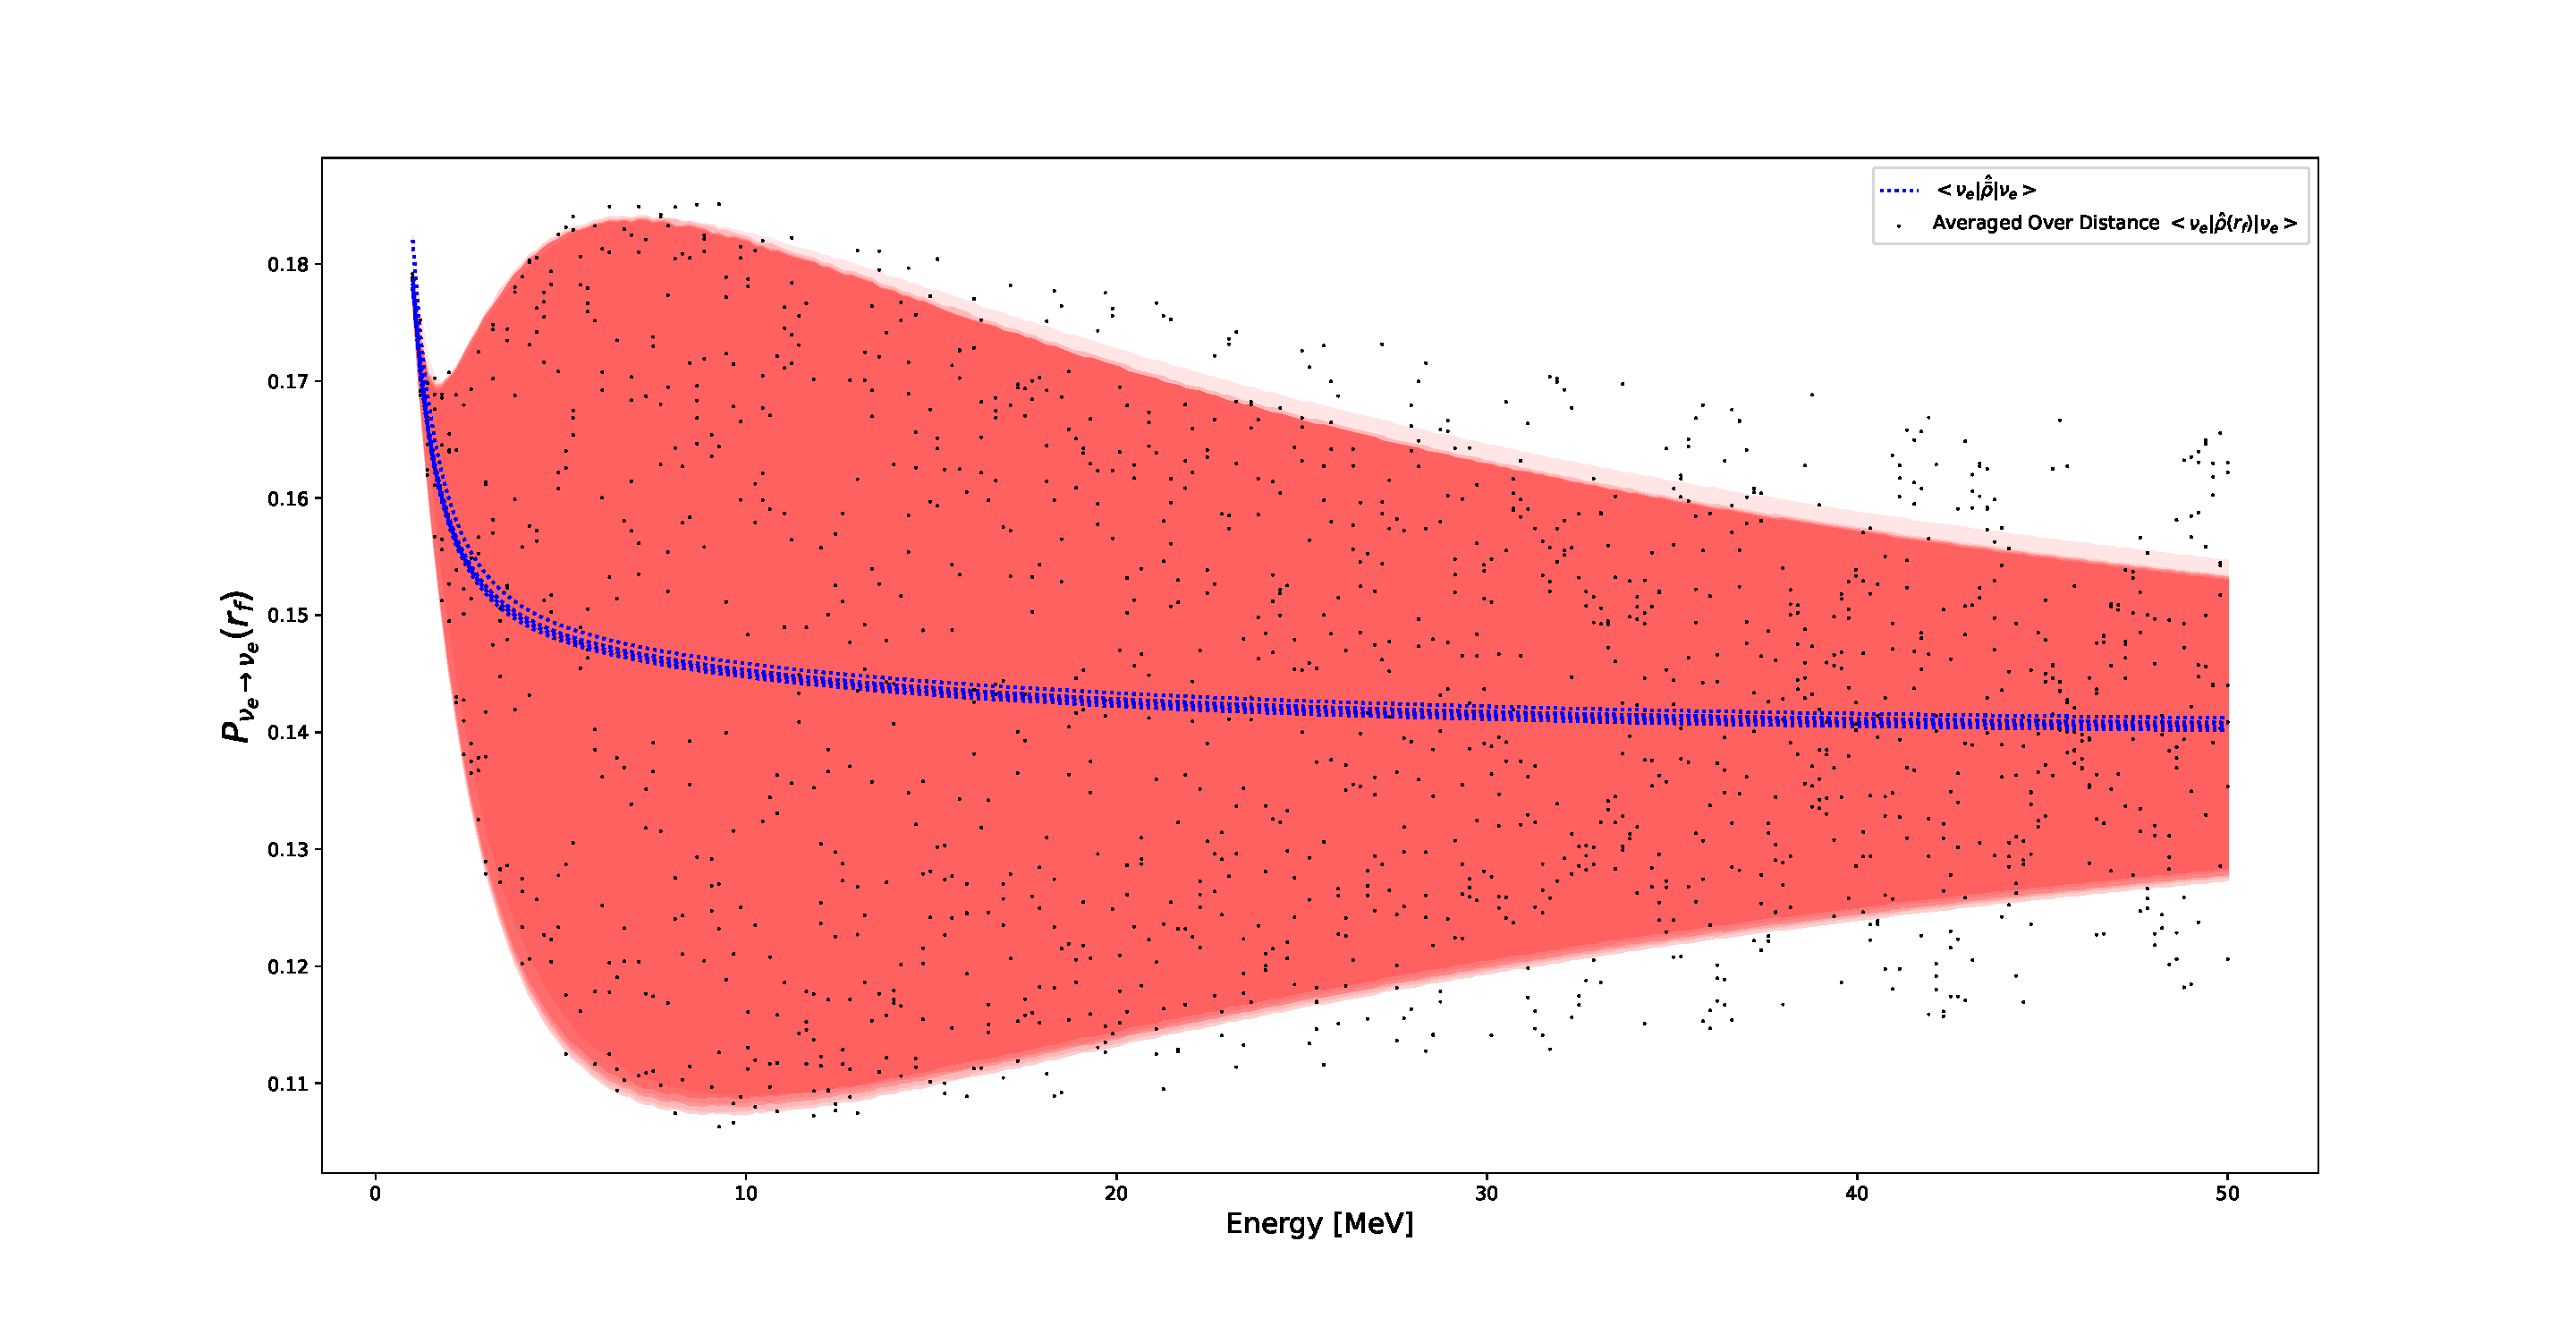
\includegraphics[width=\textwidth]{figures/theta014expNbB_energySpec_theta0_averaged.pdf}
    \caption[theta014expNbB Modeli, 9 simülasyonun Enerjiye Karşılık Yaşama Olasılıkları]{theta014expNbB Modeli,9 simülasyonun Enerjiye Karşılık Yaşama Olasılıkları. Her siyah nokta, sayısal sonuçların son birkaç kilometredeki ortalamasıdır. Boşluk karışım açısının sıfırdan farklı olması durumunda, analitik öngörü/sayısal sonuç uyumsuzluğu görülmektedir. Uyumsuzluk, yüksek enerjilerde daha belirgin hale gelmektedir.}
    \label{fig:theta014expNbB_energySpec_theta0_averaged}
\end{figure}

Eğer nötrino çeşni evriminde, bir rezonans tamamlanmadan sonraki rezonansa girer ise analitik olarak hesapladığımız ortalama yoğunluk matrisi terimi yani \eqref{eqn:rhoBar_rhoSal} numaralı denklem tam olarak doğru sonucu vermez. Bunun ilk sebebi adyabatik olmayan geçişleri veren $ A_{ij} $ terimi MSW ve SFP olmak üzere iki ayrı matrisin çarpımı olarak yazılamayacaktır. \eqref{eqn:rhoBar_hata} numaralı denklemde hata terimi türetilirken $ A_{LZ} = A_{SFP} \times A_{MSW} $ şeklinde yazıldığından dolayı elde ettiğimiz analitik öngörü formülleri tam doğru değildir. İkinci olarak ise SFP rezonansı için yazılan ve LZ geçiş olasılığını veren \eqref{eqn:LZOlasilik} numaralı formül geçerli olmayacaktır. Bunun nedeni SFP rezonansının adyabatisitesi, rezonans bölgesinde hesaplanırken efektif 2 çeşniye düşülmüştür. Bu da, rezonans bölgesinde $ \Delta \sin(2\theta) $ teriminin $ \mu B $ teriminden çok çok büyük olması varsayımında geçerlidir. theta014expNbB modelinde, $ 10 $ MeV enerjili nötrinoların tam SFP rezonansına girdiği noktada toplam Hamiltonyen'in sayısal değeri aşağıdaki gibidir. 
\begin{equation}
    H(r=840 \text{ km}) = \mqty(1.4 & -0.1 & 0 & 0.1\\ -0.1 & -2.0 & -0.1 & 0\\ 0 & -0.1 & -0.7 & -0.1\\ 0.1 & 0 & -0.1 & 1.4) ~~\text{[km}^{-1}\text{]} \text{ .}
\end{equation}
Yukarıdaki denklemden de görüleceği üzere Hamiltonyen matrisinin 12 elemanının değeri ile 14 elemanın değeri aynıdır. Bu da SFP rezonansının adyabatisite değerini bulmak için yaptığımız $ 2\times2 $ çeşni indirgenmesini olanaksız kılar. Budan dolayı $ P_{SFP} $, yanlış bir değer alır.

Analitik sonuçlar ile sayısal sonuçların uyuşmamasını daha ayrıntılı inceleyebilmemiz için iki rezonans noktası etrafındaki efektif karışım açısının sinüsünün karesine bakmak gerekmektedir, çünkü salınım ortalaması alınmış elektron yaşama olasılıkları, $ \sin^{2}(2\theta) $ ile orantılıdır \cite{Kuo:1989qe}. Buradaki $\theta $ terimi, madde etkileşimleri için $ \theta_{M} $ şeklinde, hem madde hem de elektromanyetik etkileşimler için $ \theta_{EM} $ şeklinde gelir. $ \sin^{2}(2\theta_{M}) $ ve $ \sin^{2}(2\theta_{EM}) $ terimlerinin uzaklıkla değişiminde, bu terimlerin ilgili rezonanslarda $ 1 $ değeri alacağı bilinmektedir, çünkü rezonans değerlerinde efektif karışım açısı $ \pi/4 $ değerine yaklaşacaktır. 

Efektif karışım açısının sinüsünün karesinin uzaklıkla değişimi \ref{fig:theta014expNbB_sin2_thetaM_thetaEM_dist10MeV} numaralı şekilde verilmiştir. Bu grafikte $ 40 $ MeV enerjili nötrinolar, SFP rezonansından çıkamadan MSW rezonansına girdiği gözükmektedir. Rezonansların üst üste binmesini farklı başlangıç baryon yoğunluklarına bakarak karşılaştırabiliriz. \ref{fig:theta014expNbB_sin2_thetaM_thetaEM_dist10MeV} numaralı şeklindeki en üstteki şekil, $ n_{0}=10^{6} $ g/cm$ ^{3} $ için yapılmış simülasyon sonucudur. Bu değerden daha büyük değerler alınırsa, ÇÇSN'nın daha erken dönemlerine gidilmiş olur. $ n_{0}=2.3\times 10^{6} $ g/cm$ ^{3} $ değeri $ t=3 $ s için olan evreye ve $ n_{0}=1.8\times 10^{7} $ g/cm$ ^{3} $ değeri $ t=1 $ s için olan evreye denk gelmektedir. Bunlar için analitik öngörümüzü test edebiliriz.

\begin{figure}[hbt!]
    \centering
    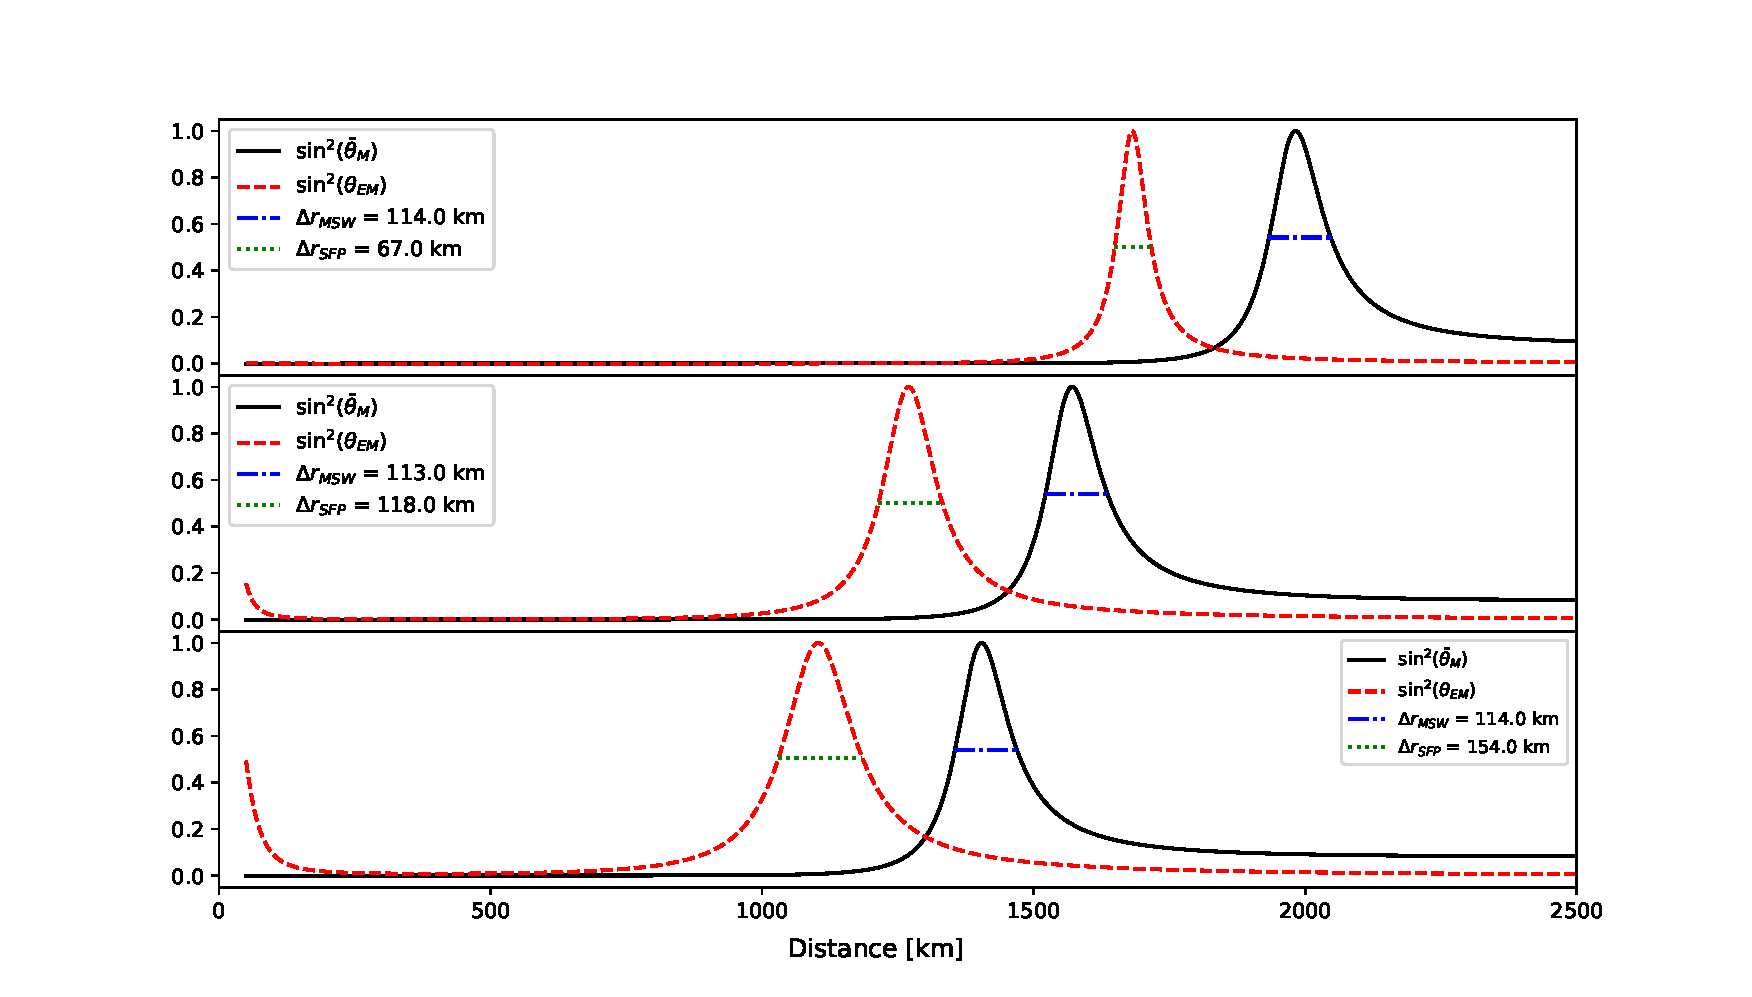
\includegraphics[width=\textwidth]{figures/widthCompare3x1_40MeV_IH_t135s.pdf}
    \caption[theta014expNbB Modelinde Rezonansların Birbirine Yakınlığı]{theta014expNbB Modelinde Rezonansların Birbirine Yakınlığı. $ \Delta r_{MSW} $ uzaklığı ile $ \Delta r_{SFP} $ uzaklığının baryon yoğunluğunun başlangıçtaki değerine göre değişimi gösterilmiştir. Şekiller, yukarıdan aşağı $ t=1 $ s, $ t=3 $ s ve $ t=5 $ s için kullanılan ÇÇSN baryon profilleri baz alınmıştır.}
    \label{fig:theta014expNbB_sin2_thetaM_thetaEM_dist10MeV}
\end{figure}

Rezonansların birbirine yakınlığı ve öngörülerimizin çalıştığı aralığı belirlemek için $ \sin^{2}(2\theta_{M}) $ ve $ \sin^{2}(2\theta_{EM}) $ terimlerinin eksponansiyel profil için analitik değerlerini hesaplamalıyız. $ \sin^{2}(2\theta) $ fonksiyonu neredeyse Gausyen bir dağılım verdiği için dağılımın yarım maksimumdaki yarım genişlik (YMYG), (half width at half maksimum, HWHM) değerleri anlamlı olacaktır. \ref{fig:theta014expNbB_sin2_thetaM_thetaEM_dist10MeV} numaralı grafikte yazan $ \Delta r_{MSW} $ ve $ \Delta r_{SFP} $ değerleri YMYG değerinin iki katıdır ve grafik üzerinden hesaplanmıştır. Bu değeri analitik olarak hesaplamak da mümkündür. $\sin^{2}(2\theta_{M}) $ teriminin yarı maksimum olduğu uzaklık, $\Delta r_{MSW}$, ifadenin $ 0.5 $'e eşit olduğu değerde olacaktır.
\begin{align}
    \sin^{2}(2\theta_{M}(\Delta r_{MSW}) ) = 0.5 = \frac{1}{1+\frac{\Delta c_{2\theta} - V_{CC}(\Delta r_{MSW})/2}{\Delta s_{2\theta}}} \text{ .}
\end{align}
Burada $ \Delta r_{MSW} $ uzaklığı, maksimum değerinin etrafında, iki farklı değerde olacaktır. Bu uzaklıklar, $ n_{b}(r) = n_{0}\exp(-r/r_{mat}) $ profili için aşağıdaki değerleri alır.
\begin{equation}
    r^{MSW}_{hm1}, r^{MSW}_{hm2} = (-r_{mat})\ln(\frac{1}{n_{0}}\frac{\Delta c_{2\theta} \pm \Delta s_{2\theta}}{\sqrt{2} G_{F} Y_{e}/2}) \text{ .}
\end{equation}
MSW rezonansının meydana geldiği noktadaki yarım genişlik $ r^{MSW}_{hw} $, MSW rezonansının kaç kilometre boyunca meydana geldiğini betimleyen bir büyüklük olarak karşımıza çıkar ve bu değer aşağıdaki gibi tanımlanır.
\begin{align} \label{eqn:rMSW_hw}
    \nonumber \Delta r_{MSW}/2 =& \abs{r^{MSW}_{hm1}- r^{MSW}_{hm2}}/2 \text{ ,}\\
    =& \frac{-r_{mat}}{2} \ln(\frac{c_{2\theta} - s_{2\theta}}{c_{2\theta} + s_{2\theta}}) \text{ .}
\end{align}
Bu ifadeden de görüleceği üzere, MSW rezonansının genişliği enerjiden, kütle kare farkından ve baryon yoğunluğunun başlangıçtaki değerinden bağımsızdır. 

Benzer işlemleri SFP rezonansı için de yapabiliriz. Manyetik alanın $ B(r) = B_{0}(50 \text{ km}/r)^{2} $ şeklinde alınacaktır. SFP rezonansının gerçekleştiği yarı maksimum uzaklıkları aşağıdaki denklemlerin çözümü ile verilir.
\begin{align}
    \Delta c_{2\theta} - \frac{2Y_{e}-1}{2}\sqrt{2}G_{F}n_{0}e^{-\Delta r_{SFP}/r_{mat}}\pm \mu B_{0}(50 \text{ km}/\Delta r_{SFP})^{2} = 0\text{ .}
\end{align}
Bu denklemin $ \Delta r_{SFP} $ için çözümü yoktur. Bunun yerine rezonans bölgesinde manyetik alanın neredeyse sabit ve $ B_{1} $ değeri aldığını varsayacağız. Bu yaklaşıklık altında yarım genişlik $ \Delta r_{SFP}/2 $ değeri aşağıdaki gibi hesaplanır.
\begin{equation}\label{eqn:rSFP_hw}
    \Delta r_{SFP}/2 = \frac{-r_{mat}}{2} \ln(\frac{\Delta c_{2\theta}-\mu B_{1}}{\Delta c_{2\theta}+\mu B_{1}})\text{ .}
\end{equation}
Bu ifade, $ r^{MSW}_{hw} $ genişliğinden farklı olarak enerjiye, kütle kare farkına ve manyetik alana da bağlıdır. \eqref{eqn:rMSW_hw} ve \eqref{eqn:rSFP_hw} numaralı denklemlerden elde edilen YMYG ile \ref{fig:theta014expNbB_sin2_thetaM_thetaEM_dist10MeV} numaralı şekilden elde edilen YMYG değeri farklı olacaktır. Örneğin karışma açısı büyüdükçe, $ \sin^{2}(2\theta_{M}) $ ifadesinin grafikten elde edilen yarı maksimumun değeri $ 0.5 $'ten uzaklaşacaktır. Ayrıca \ref{fig:theta014expNbB_sin2_thetaM_thetaEM_dist10MeV} numaralı şekilden MSW rezonansının YMYG değeri, $ n_{0} $'dan bağımsız olduğu gözükmektedir.

Rezonansların birbirine ne kadar yakın olduklarını sayısal bir değer tanımlayarak belirleyebiliriz. Bunun için \ref{fig:theta014expNbB_sin2_thetaM_thetaEM_dist10MeV} numaralı şekildeki Gausyen dağılımın YMYG değeri bize bir fikir verecektir. \cite{Smirnov:2003da} numaralı kaynağın 6 numaralı şeklinde, rezonansın başlangıç ve bitiş noktaları rezonansın meydana geldiği noktadan yaklaşık $3$ adet YMYG değeri kadar uzaklarda "bittiği" anlaşılmaktadır. Eğer, rezonansların birbirlerine olan uzaklığının, yarı uzaklık toplamlarına oranı sıfıra yaklaşırsa rezonanslar üst üste geliyor demektir. \ref{fig:theta014expNbB_sin2_thetaM_thetaEM_dist10MeV} numaralı grafikteki değerler için bu oranları yazabiliriz.
\begin{align}\label{eqn:resonansYakinlasmaOranı}
    \eval{\frac{\abs{r^{SFP} - r^{MSW}}}{r^{SFP}_{hw}+r^{MSW}_{hw}}}_{t=1,3,5 \text{ s}} = 3.31\text{, } 2.60\text{, } 2.24 \text{ .}
\end{align}
Yukarıdaki değerlere bakınca, ÇÇSN erken evrelerinde (başlangıç baryon yoğunluk değeri arttıkça) rezonansların birbirinden daha ayrı olduğunu söyleyebiliriz. ÇÇSN evriminde zaman ilerledikçe rezonanslar birbirine yaklaşmaktadır. Rezonansların birbirine yaklaşması üç çeşni etkilerinin ortaya çıkması anlamına da gelir.

Çeşni evrimindeki üç çeşni etkilerini başka bir parametre ile de görmek mümkündür. SFP rezonansının başladığı sırada, \eqref{eqn:Hamiltonyen_withGamma} numaralı Hamiltonyen'i üç çeşniye indirgeyelim. Bu Hamiltonyen, madde tabanında yazıldığı için seçeceğimiz üç terim, başlangıç koşullarına bağlıdır. Bizim notasyonumuza göre, ters hiyerarşi ve $ Y<0.5 $ başlangıç koşulları için indirgenmesi gereken terimler $ \omega_{1,2,4} $ ve bunlarla alakalı olan terimler olacaktır.

\begin{equation}
    H_{3\times3} = \mqty(\omega_{1} & \mu B \sin\gamma & \mu B \cos \gamma \\ \mu B \sin\gamma & \omega_{2} & \mu B \sin \gamma \\ \mu B \cos \gamma & \mu B \sin\gamma & \omega_{4}) \text{ .}
\end{equation}

Salınım etkilerinin olmadığı durumlarda, $ \theta=0 $, efektif madde karışım açı farkı $ \gamma=0 $ olur. Bu durumda geçişler sadece $ \omega_{1} $ ile $ \omega_{4} $ arasında olacaktır. Başlangıçta, birinci öz durum çoğunlukla elektron, dördüncü öz durum çoğunlukla anti $x$ çeşnisi olduğu düşünüldüğünde, bu geçişler SFP rezonansına sebep olacaktır.

Boşluk salınım açısının sıfırdan farklı olduğu durumda ise SFP rezonansı sırasında köşegen olmayan terimler sıfır olmayacak. Yani $ \mu B \sin \gamma \ne 0 $ şeklinde olacaktır. Bir diğer taraftan, SFP rezonansının meydana geldiği uzaklıkta $ \omega_{1}-\omega_{4} $ neredeyse sıfır olacaktır. Bu noktadaki üç çeşniye indirgenmiş Hamiltonyen'i tekrar yazalım. Hamiltonyen'i yazarken $ \omega_{4} $ ile birim matris çarpımını Hamiltonyen'den çıkaralım. 
\begin{equation}
    H_{3\times3}(r_{SFP}) = \mqty(0 & \mu B \sin\gamma & \mu B \cos \gamma \\ \mu B \sin\gamma & \omega_{2}(r_{SFP})-\omega_{4}(r_{SFP}) & \mu B \sin \gamma \\ \mu B \cos \gamma & \mu B \sin\gamma & 0) \text{ .}
\end{equation}
Sistem SFP rezonansına girerken, özdurum geçişleri sadece $ \omega_{1} $ ile $ \omega_{4} $ arasında olmayacaktır. $ \mu B \sin \gamma $ teriminden kaynaklı $ \omega_{2} $ ile $ \omega_{4} $ arasında da olacaktır. Bu nedenle, iki çeşniye indirgenerek elde edilen tüm parametreler düzgün çalışmaz. 

Yukarıda bahsedilen, özdurumlar arasındaki bu \emph{sızma} (leaking) olayının büyüklüğünü, sızma parametresi $ L $ terimini tanımlayarak belirleyebiliriz.
\begin{equation}
    L = \eval{\frac{\mu B \sin \gamma}{\omega_{i}-\omega_{j}}}_{r_{SFP}}
\end{equation}

theta014expNbB başlangıç koşulları kullanıldığında $ i,j = 2,4 $ olacaktır. \textit{Sızma parametresi ne kadar küçük olursa üç çeşni etkileri o kadar az olur.} theta014expNbB simülasyonu için $ L $ parametresi $ 20 $ civarındadır. Sızma parametresi $ 5 $ civarında iken üç çeşni etikleri çok küçüktür ve öngörü/simülasyon sonuçları tam olarak uyumlu çıkar. Sızma parametresi için söylenecek son söz ise boşluk karışım açısı $ \theta $ arttığında veya başlangıçtaki madde yoğunluğu azaldığında $ L $ değeri büyüyecektir. 

Sonuç olarak \eqref{eqn:rhoBar_ort} ve \eqref{eqn:rhoBar_hata} numaralı denklemler ancak ve ancak \eqref{eqn:resonansYakinlasmaOranı} numaralı bağıntıda verilen oran $ 3 $'ten büyük ise veya $ L \sim 5$ olduğunda kullanılabilir. Elde ettiğimiz bu iki koşul birbiriyle ilişkilidir. 

Elde ettiğimiz öngörüleri ve geçerli olduğu başlangıç koşulları kullanarak ÇÇSN'nın $ t=1 $ s ve $ t=3 $ s evrelerinde yaşama olasılıklarını belirleyebiliriz. Enerjiye bağlı son yaşama olasılıkları 
$ t=1 $ s için \ref{fig:theta014expNbB_t1s_energySpec_theta0_averaged} numaralı şekilde ve $ t=3 $ s için \ref{fig:theta014expNbB_t3s_energySpec_theta0_averaged} numaralı grafikte belirlenmiştir. Öngördüğümüz gibi zaman azaldıkça analitik sonuçlar ve sayısal sonuçlar üst üste oturmaktadır. Tüm bu hesapları normal hiyerarşi için de yaptık ve benzer sonuçlar elde ettik.

\begin{figure}[hbt!]
    \centering
    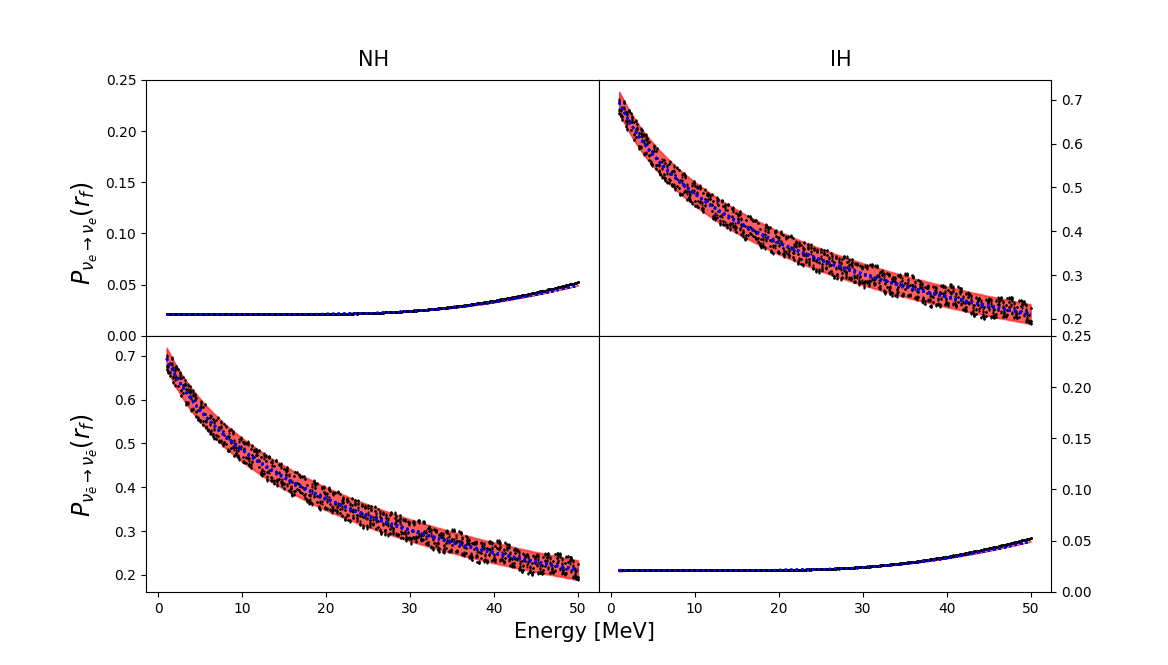
\includegraphics[width=\textwidth]{figures/theta014expNbB_t1s_energySpec_theta0_averaged.png}
    \caption[$ t=1 $ s başlangıç koşullu, theta014expNbB Modeli, 9 simülasyonun Enerjiye Karşılık Yaşama Olasılıkları.]{$ t=1 $ s başlangıç koşullu, theta014expNbB Modeli, 9 simülasyonun Enerjiye Karşılık Yaşama Olasılıkları. Her siyah nokta, sayısal sonuçların son birkaç kilometredeki ortalamasıdır. Normal hiyerarşi ile yapılan simülasyonlarda başlangıçta sadece elektron antinötrinosu bulunmaktadır. Başlangıç baryon yoğunluğu $ n_{0}=1.8\times 10^{7} $ g/cm$ ^{3} $ değerindedir.}
    \label{fig:theta014expNbB_t1s_energySpec_theta0_averaged}
\end{figure}

\begin{figure}[hbt!]
    \centering
    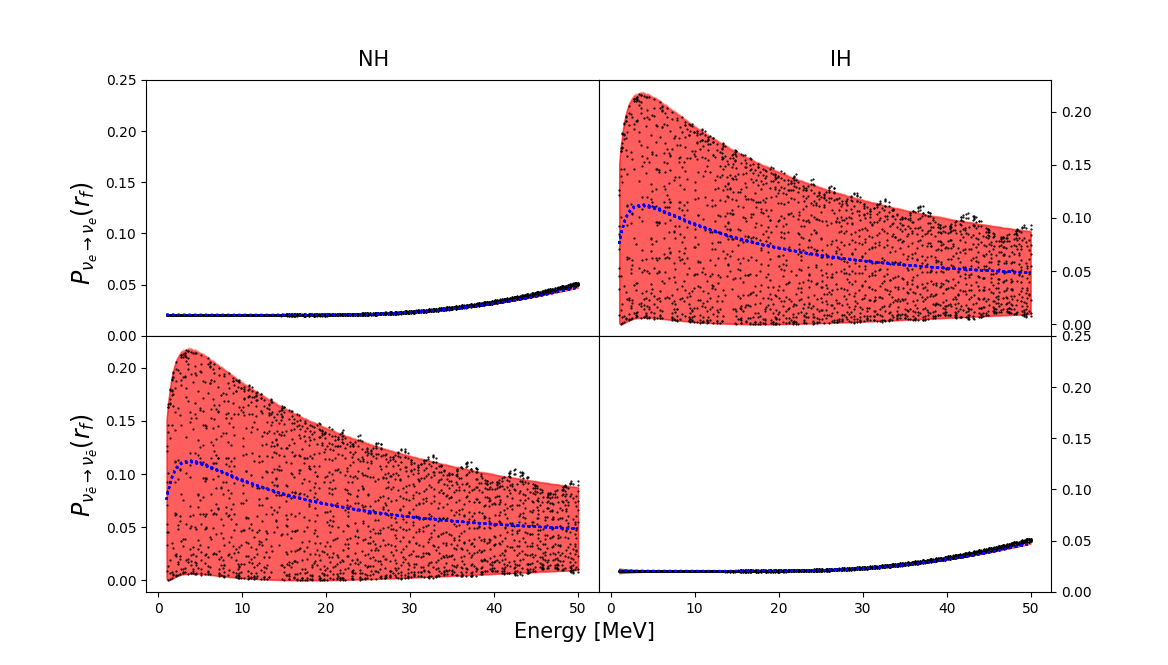
\includegraphics[width=\textwidth]{figures/theta014expNbB_t3s_energySpec_theta0_averaged.png}
    \caption[$ t=3 $ s başlangıç koşullu, theta014expNbB Modeli, 9 simülasyonun Enerjiye Karşılık Yaşama Olasılıkları.]{$ t=3 $ s başlangıç koşullu, theta014expNbB Modeli, 9 simülasyonun Enerjiye Karşılık Yaşama Olasılıkları. Her siyah nokta, sayısal sonuçların son birkaç kilometredeki ortalamasıdır. Normal hiyerarşi ile yapılan simülasyonlarda başlangıçta sadece elektron antinötrinosu bulunmaktadır. Başlangıç baryon yoğunluğu $ n_{0}=2.3\times 10^{6} $ g/cm$ ^{3} $ değerindedir.}
    \label{fig:theta014expNbB_t3s_energySpec_theta0_averaged}
\end{figure}

$ Y_{e}$ değiştiğinde MSW ve SFP rezonanslarının konumu değişir (bakınız \ref{fig:resonance_nb_Ye} numaralı şekil.) Özellikle $ Y_{e}$ değeri  $ 0.5 $ değerine yaklaştıkça rezonanslar birbirinden uzaklaşır. Bu başlangıç koşulu kurulumunda ise $ P_{SFP} $ değeri çok küçük çıkar ve SFP rezonansı adyabatik bir geçiş olur. Adyabatik geçişler de başlangıç koşullarındaki küçük değişimlerden bağımsızdır. Başka türlü ifade etmek gerekirse 9 farklı simülasyonun analitik öngörüsü aynı çıkar. Bu bölümde, kırmızı ile belirtilen hata aralığı sıfır olur ve fazların etkisi yok olur.

\section{GERÇEKÇİ MODELLER}\label{sec:gercekciModeller}
Bu bölümde, gerçekçi bir ÇÇSN modeli kullanarak simülasyonlar yapılacaktır. Yapılan simülasyonlarda nötrino elektromanyetik etkileşimin ve nötrino öz-kırılımının kollektif nötrino salınımına olan etkisi incelenecektir. Bir önceki bölümün aksine bu bölümde baryon yoğunluğu ÇÇSN modelinden alınacaktır. Özel olarak $ t=0 $ s'deki yoğunluk \cite{1987ESOC...26..325N} numaralı referanstaki SN1987A modelinden alınacak, onun üzerine \cite{Athar:1995cx} numaralı referansta tarif edilen şekilde parametrik bir şok dalgası eklenerek $ t>0 $ anlarındaki yoğunluklar elde edilecektir. Manyetik alan ise \ref{tab:simulasyonlar} numaralı tabloda verildiği gibi alınacaktır.

Baryon yoğunluğunu ve elektron kesrini veren grafik \ref{fig:t5s_nbYe2dist} numaralı şekilde verilmiştir. Tüm simülasyonlar bu profile göre yapılmıştır.

\begin{figure}[hbt!]
    \centering
    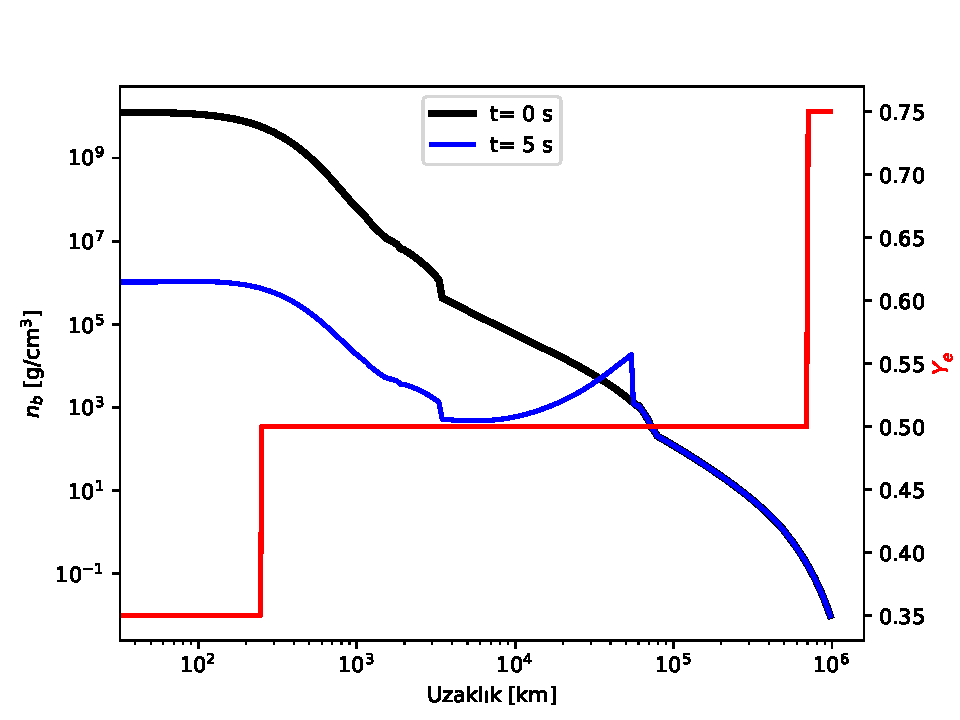
\includegraphics[width=0.9\textwidth]{figures/t5s_nbYe2dist.pdf}
    \caption[$ t=5 $s İçin Baryon Yoğunluğu ve Elektron Kesri.]{$ t=5 $s İçin Baryon Yoğunluğu ve Elektron Kesri. Yaklaşık $250$ km'de elektron kesri aniden yükselmektedir. Şok dalgasının konumu ise $55000$ km civarındadır.}
    \label{fig:t5s_nbYe2dist}
\end{figure}

ÇÇSN oluşmadan önce merkeze yakın noktalarda nötron fazlalığı bulunmaktadır \cite{Athar:1995cx}. Bu nötron fazlalığı elektron kesrini $ 0.5 $ değerinden daha küçük bir değere getirecektir. Patlama gerçekleştikten sonra açığa çıkan şok dalgası ile beraber bu nötron yoğunluğu olan bölge daha iç bölgelere taşınacaktır. Bu tezde nötron zengin bölgeyi $ 50 $ ile $ 250 $ km arasında alacağız. Bu değer bir önceki bölümdeki süreksizliğin olduğu $ r_{d} $ uzaklığına denktir. Pre-süpernova fazındayken $ r_{d} $ değeri yaklaşık $ 10^{-3} R_{\odot} $ uzaklığındadır \cite{Athar:1995cx}. Son olarak, not edilmelidir ki bu nötron zengin bölgede $ r $-işlem (r-process, rapid process) çekirdek sentezi meydana gelmektedir \cite{Janka:2006fh,Arnould:2007gh,Qian:1996xt}.

Gerçekçi simülasyonlarda ortak olan bir diğer nicelik ise nötrino parlaklığıdır. Nötrino parlaklığı, süpernova evresine yani zamana bağlı olarak düşecektir. Bu düşme aşağıdaki gibi parametrize edilir.
\begin{equation}
    L(t)= L_{0}\exp(-t/\tau)
\end{equation}
Burada $ \tau=3 $ olarak alınmıştır \cite{2017hsn..book.1605R, Mirizzi:2015eza}. $ L_{0} $ total bağlanma enerjisinden bulunabilir ve yapılan SN simülasyonuna bağlıdır. Bu çalışmada bağlanma enerjisi yaklaşık $ 10^{53} $ erg civarında seçilmiştir. Buna bağlı olarak $ L_{0}=10^{52} $ erg/s olacaktır. Bu değerler SN1987A modelini ortaya koyan çalışmalarla uyumludur \cite{fukugita2013physics}. $ t=1 $ s için $ 0.7 $ katına, $ t=5 $ s. için $0.26$ katına düşecektir. Tüm nötrino çeşnileri için aynı parlaklık değeri kullanılmıştır.

Nötrino dağılımları ise Fermi-Dirac dağılımı olarak alınacaktır. Nötrino sıcaklıkları ise $ T_{\nu_{e}}=3 $, $T_{\nu_{\bar{x}}}=4 $ ve $T_{\nu_{\bar{x}},\nu_{x}}=6 $ MeV değerleri alınmıştır. Bunun dışındaki diğer temel parametreler, son uzaklık ve nötrino istatistiksel dağılım dışında, \ref{tab:oyuncakModOrtakBasKos} numaralı tabloda verilmiştir. Ayrıca $ \delta m^{2}= 2.56 \times 10^{-15} $ MeV alınmıştır \cite{ParticleDataGroup:2018ovx}.

Aşağıdaki, \ref{fig:t5sNoCollnuNoB_distdiag10}, \ref{fig:t5sNoCollnuNoB_spectrum}, \ref{fig:t5sNoCollnuB_distdiag10}, \ref{fig:t5sNoCollnuB_spectrum} , \ref{fig:t5sCollnuNoB_distdiag10}, \ref{fig:t5sCollnuNoB_spectrum}, \ref{fig:t5sCollnuB_distdiag10} ve \ref{fig:t5sCollnuB_spectrum} numaralı grafiklerin hepsinde aynı renk kodu kullanılmıştır. Siyah renk elektron çeşnisine, mavi renk $ x $ çeşnisine, kırmızı renk anti elektron çeşnisine ve yeşil renk ise anti $ x $ çeşnisine denk gelmektedir. Spektrum grafikleri, çeşni evriminin başlangıçtaki ve simülasyonun sonundaki durumlarını gösterir. Simülasyonlar $ 70000 $ km'ye kadar yapılmıştır. Bu uzaklıktan sonra nötrinoların çeşni evrimini etkileyen bir olay olmamaktadır, yani, nötrinolar efektif olarak boşluğa ulaşmıştır diyebiliriz. Ayrıca antinötrinoların spektrumu ile nötrinoların spektrumu karışmaması için antinötrinoların spektrumu negatif enerjili gibi gösterilmiştir.

Tüm modellerde, ters hiyerarşi dikkate alındığı için MSW rezonansı antinötrino çeşnileri arasında gerçekleşecektir. 

\textbf{t5sNoCollnuNoB} adlı simülasyonda sadece nötrino madde etkileşimi dikkate alınmıştır. $ 10 $ MeV enerjileri nötrinoların uzaklığa göre çeşni evrimi \ref{fig:t5sNoCollnuNoB_distdiag10} numaralı şekilde, enerjiye göre spektrumuları ise \ref{fig:t5sNoCollnuNoB_spectrum} numaralı şekilde gösterilmektedir. $ 250 $ km uzaklığına kadar elektron kesri $ 0.35 $ değerinde olduğu için antinötrinolar bu bölgede bir adet rezonansa girmektedir. Ardından elektron kesri $ 0.5 $ değeri almıştır. Bu değeri aldığında ise antinötrinolar yaklaşık $ 30000 $ km'de tekrar MSW rezonansına girer. Son olarak $ 55000 $ km'de nötrinolar şok dalgası ile karşılaşır. Bu noktada baryon yoğunluğu yükseldiği için üçüncü MSW rezonansı meydana gelmektedir. Elektron ve $ x $ nötrinolarında ise girilen rezonansın adyabatikliğinden sapma oranında değişimler gözükmektedir. \ref{fig:t5sNoCollnuNoB_spectrum} numaralı şekilden görüldüğü üzere, meydana gelen tüm rezonanslar sadece $ 10 $ MeV için değil tüm antinötrinolara etki etmektedir. Bu durum $ t<5 $ s için geçerli değildir. Daha yüksek baryon yoğunluklarında, sadece yüksek enerjili nötrinolar üçüncü rezonansa girecektir \cite{Ekinci:2021miy}.

\textbf{t5sNoCollnuB} adlı simülasyonda nötrino madde etkileşimi ve nötrino elektromanyetik etkileşimi dikkate alınmıştır. $ 10 $ MeV enerjileri nötrinoların uzaklığa göre çeşni evrimi \ref{fig:t5sNoCollnuB_distdiag10} numaralı şekilde, enerjiye göre spektrumuları ise \ref{fig:t5sNoCollnuB_spectrum} numaralı şekilde gösterilmektedir. Başlangıçtaki yüksek manyetik alan elektron nötrinosu ve $ x $ antinötrinosunu karıştıracaktır. Çeşni bazında bakıldığında temiz bir MSW ve SFP rezonansı meydana gelmemektedir. Bir diğer taraftan $ x $ nötrinosu, etkileşimlerden etkilenmeden ayrışacaktır. \ref{fig:t5sNoCollnuB_spectrum} numaralı spektrum şekli, çeşni evrimi sonlandığında elektron nötrinosunun bir kısmının $ x $ antinötrinosuna geçtiğini gösterir. Bunun sebebi $ 250 $ km'ye kadar etkisini gösteren elektromanyetik alan etkileşimleridir. Eğer $ 250 $ km'den sonrasında elektron kesri $ 0.5 $ yerine $ 0.5 $'ten çok küçük farklı alınsaydı SFP rezonansı da meydana gelir. Nötrino öz-kırılımı dikkate alınmadığında, $ x $ antinötrinosunun ile elektron antinötrinosu aynı sıcaklığa geldiğini söyleyebiliriz. Bu "yeni" sıcaklığı veren elektron nötrinosudur. Elektron nötrinosunun sıcaklığının düşmesi ÇÇSN dinamiklerini değiştirebilir.

\textbf{t5sCollnuNoB} adlı simülasyonda nötrino madde etkileşimi ve nötrino öz-kırılımı dikkate alınmıştır. $ 10 $ MeV enerjileri nötrinoların uzaklığa göre çeşni evrimi \ref{fig:t5sCollnuNoB_distdiag10} numaralı şekilde, enerjiye göre spektrumuları ise \ref{fig:t5sCollnuNoB_spectrum} numaralı şekilde gösterilmektedir. Nötrino öz-kırılımının doğrusal olmayan etkileri \ref{fig:t5sCollnuNoB_distdiag10} numaralı şekilden gözükmektedir. Elektron ve $ x $ nötrinoları başlangıçta çok hızlı salınmaktadır. Antinötrinoların çeşni salınım genlikleri nötrinolar kadar fazla değildir ve MSW rezonansına girişleri açıkça gözükür. \ref{fig:t5sCollnuNoB_spectrum} numaralı spektrum grafiğinde ise iki adet temiz spektral yer değiştirme davranışı gözükmektedir. Spektral yer değiştirmeler nötrinolar için $ 9 $ MeV'de, antinötrinolar için $ 11 $ MeV'de gözükmektedir. Antinötrinolar MSW rezonansına da girdiği için $ 11 $ MeV'den düşük enerjili antinötrinoların spektrumları hali hazırda yer değişmiş bulunmaktadır.

\textbf{t5sCollnuB} adlı simülasyonda nötrino madde etkileşimi, nötrino öz-kırılımı ve nötrino elektromanyetik etkileşimi dikkate alınmıştır. $ 10 $ MeV enerjileri nötrinoların uzaklığa göre çeşni evrimi \ref{fig:t5sCollnuB_distdiag10} numaralı şekilde, enerjiye göre spektrumuları ise \ref{fig:t5sCollnuB_spectrum} numaralı şekilde gösterilmektedir. Bu model en gerçekçi modeldir. t5sCollnuNoB modeli ile karşılaştırıldığında manyetik momentin çeşni evrimine olan katkısı görülebilir. \ref{fig:t5sCollnuB_distdiag10} numaralı şekil ile \ref{fig:t5sCollnuNoB_spectrum} numaralı şeklin birbirinden en önemli farkı antinötrinoların spektral yer değiştirmesi kaybolmuş veya gizlenmiştir. Manyetik alan, $ x $ antinötrinoların sıcaklığını arttığından dolayı yer değiştirme kaybolmuştur. Bir diğer taraftan nötrinoların $ 9 $ MeV'de başlayan spektral yer değiştirme davranışı elektron nötrinoları için tamamlanmış ancak $ x $ antinötrinosu için tamamlanmamıştır.

\newpage
\begin{figure}[hbt!]
    \centering
    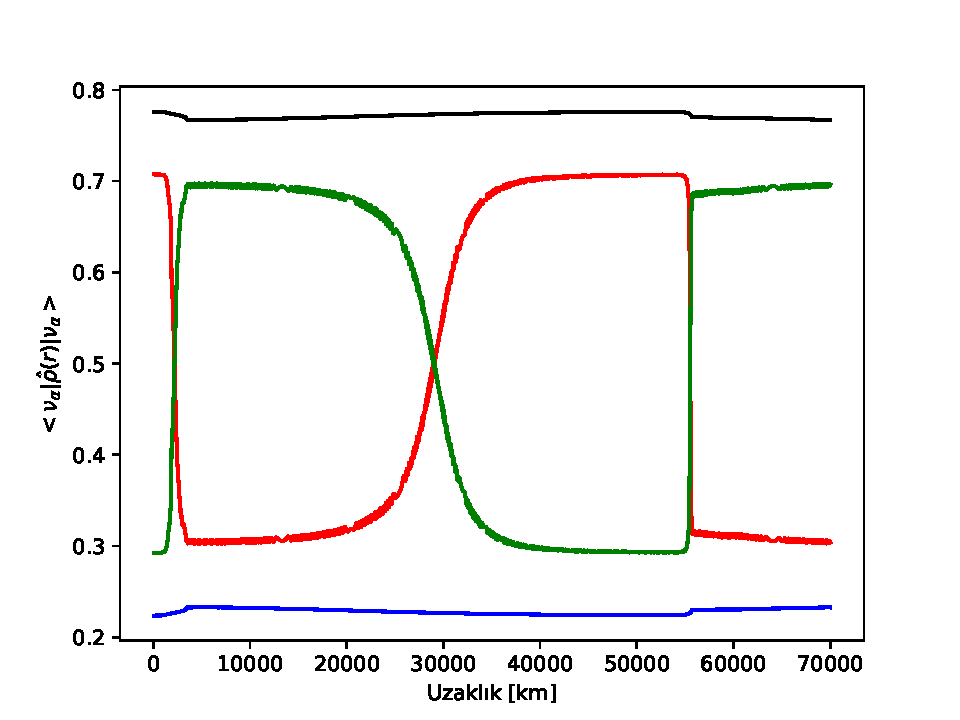
\includegraphics[width=0.9\textwidth]{figures/t5sNoCollnuNoB_distdiag10.pdf}
    \caption[t5sNoCollnuNoB Modeli, Yoğunluk Matrisinin Köşegen Elemanlarının Uzaklığa Göre Değişimi.]{t5sNoCollnuNoB Modeli, Yoğunluk Matrisinin Köşegen Elemanlarının Uzaklığa Göre Değişimi. Renk kodu: Siyah $ \nu_{e} $, mavi $ \nu_{x} $, kırmızı $ \nu_{\bar{e}} $, yeşil $ \nu_{\bar{x}} $}
    \label{fig:t5sNoCollnuNoB_distdiag10}
\end{figure}
\begin{figure}[hbt!]
    \centering
    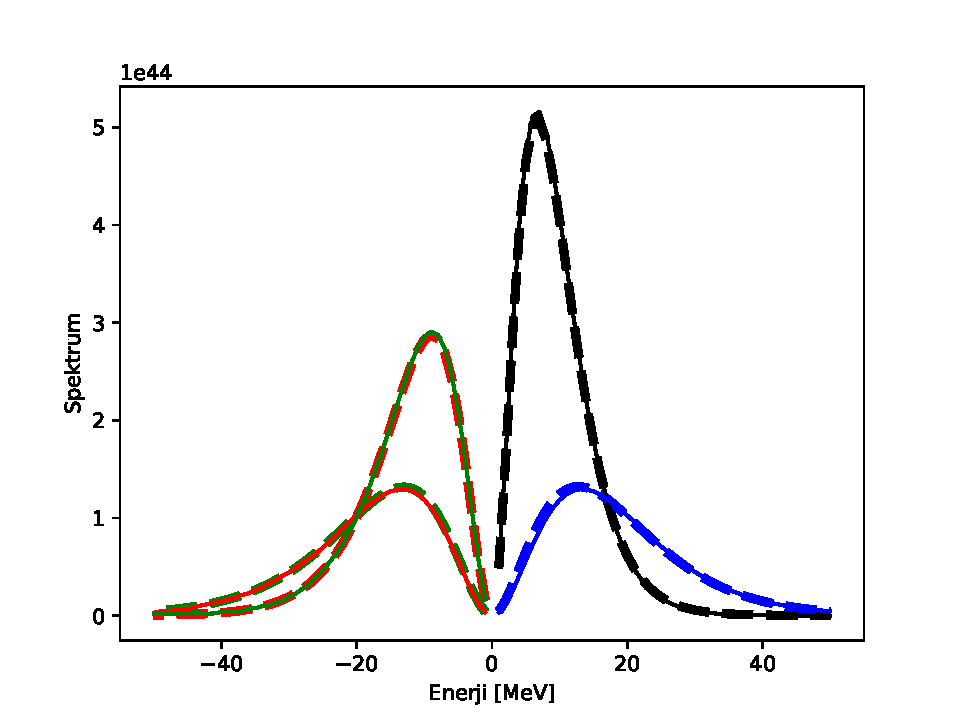
\includegraphics[width=0.9\textwidth]{figures/t5sNoCollnuNoB_spectrum.pdf}
    \caption[t5sNoCollnuNoB Modeli, Enerji Spektrumu.]{t5sNoCollnuNoB Modeli, Enerji Spektrumu. Renk kodu: Siyah $ \nu_{e} $, mavi $ \nu_{x} $, kırmızı $ \nu_{\bar{e}} $, yeşil $ \nu_{\bar{x}} $}
    \label{fig:t5sNoCollnuNoB_spectrum}
\end{figure}

\newpage
\begin{figure}[hbt!]
    \centering
    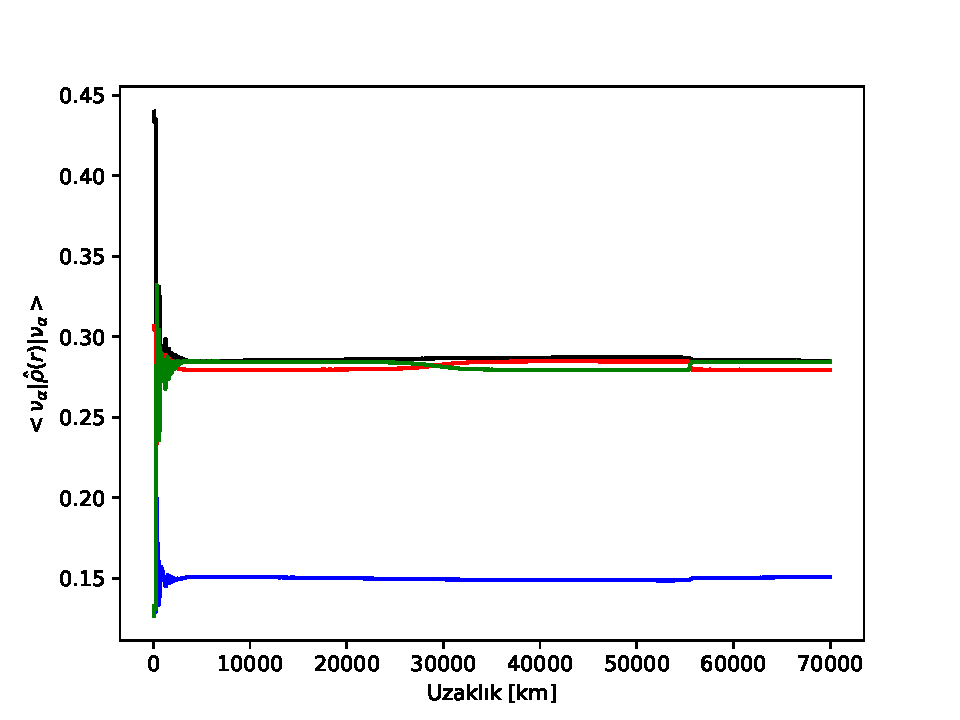
\includegraphics[width=0.9\textwidth]{figures/t5sNoCollnuB_distdiag10.pdf}
    \caption[t5sNoCollnuB Modeli, Yoğunluk Matrisinin Köşegen Elemanlarının Uzaklığa Göre Değişimi.]{t5sNoCollnuB Modeli, Yoğunluk Matrisinin Köşegen Elemanlarının Uzaklığa Göre Değişimi. Renk kodu: Siyah $ \nu_{e} $, mavi $ \nu_{x} $, kırmızı $ \nu_{\bar{e}} $, yeşil $ \nu_{\bar{x}} $}
    \label{fig:t5sNoCollnuB_distdiag10}
\end{figure}
\begin{figure}[hbt!]
    \centering
    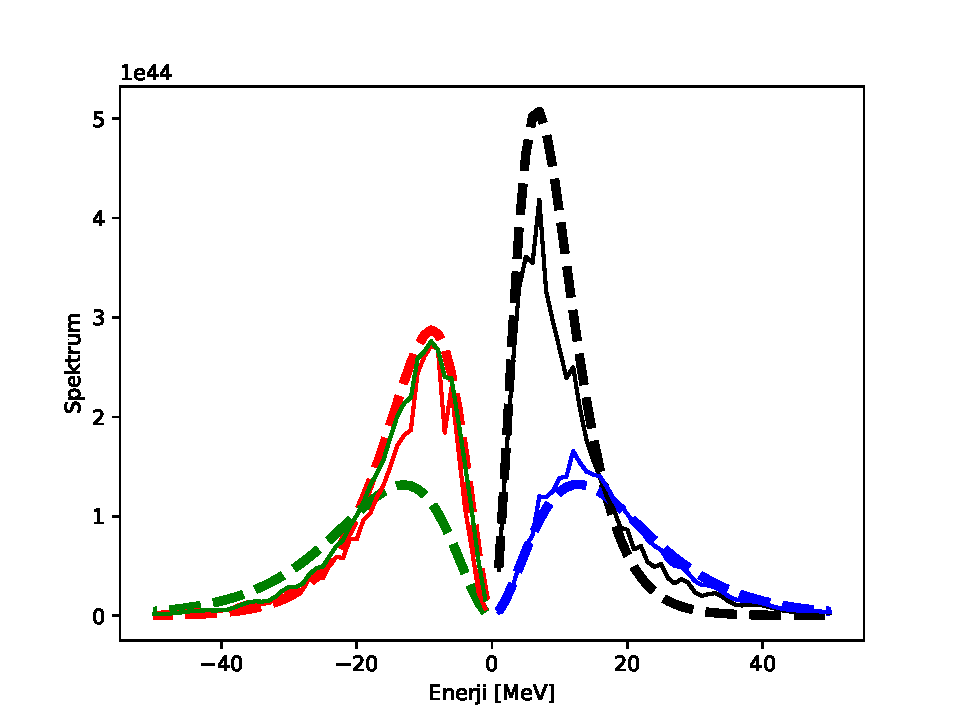
\includegraphics[width=0.9\textwidth]{figures/t5sNoCollnuB_spectrum.pdf}
    \caption[t5sNoCollnuB Modeli, Enerji Spektrumu.]{t5sNoCollnuB Modeli, Enerji Spektrumu. Renk kodu: Siyah $ \nu_{e} $, mavi $ \nu_{x} $, kırmızı $ \nu_{\bar{e}} $, yeşil $ \nu_{\bar{x}} $}
    \label{fig:t5sNoCollnuB_spectrum}
\end{figure}

\newpage
\begin{figure}[hbt!]
    \centering
    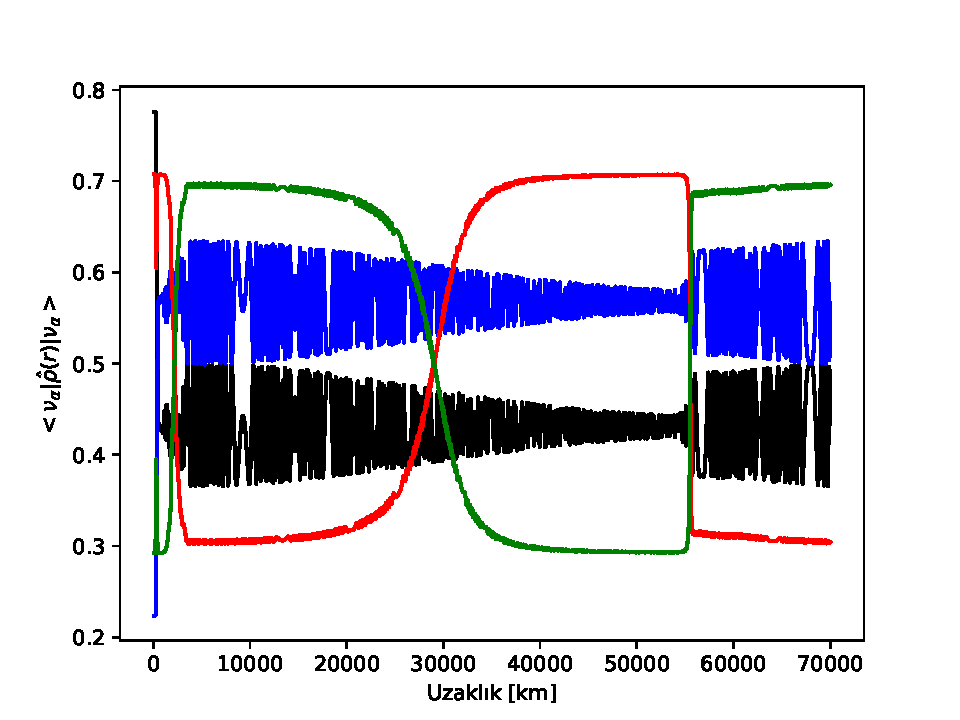
\includegraphics[width=0.9\textwidth]{figures/t5sCollnuNoB_distdiag10.pdf}
    \caption[t5sCollnuNoB Modeli, Yoğunluk Matrisinin Köşegen Elemanlarının Uzaklığa Göre Değişimi.]{t5sCollnuNoB Modeli, Yoğunluk Matrisinin Köşegen Elemanlarının Uzaklığa Göre Değişimi. Renk kodu: Siyah $ \nu_{e} $, mavi $ \nu_{x} $, kırmızı $ \nu_{\bar{e}} $, yeşil $ \nu_{\bar{x}} $}
    \label{fig:t5sCollnuNoB_distdiag10}
\end{figure}
\begin{figure}[hbt!]
    \centering
    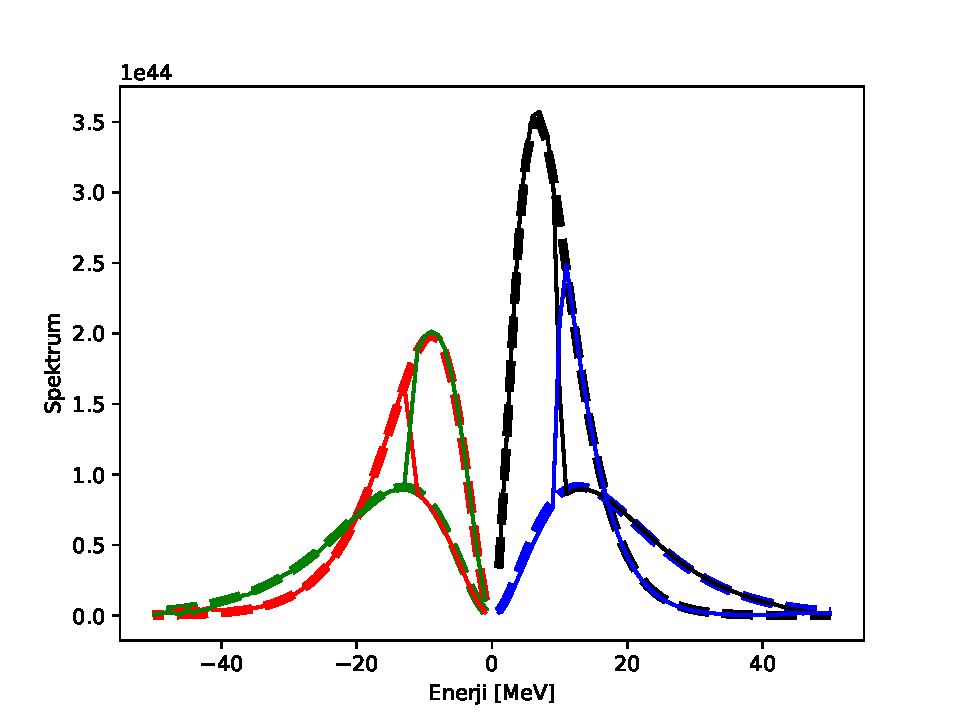
\includegraphics[width=0.9\textwidth]{figures/t5sCollnuNoB_spectrum.pdf}
    \caption[t5sCollnuNoB Modeli, Enerji Spektrumu.]{t5sCollnuNoB Modeli, Enerji Spektrumu. Renk kodu: Siyah $ \nu_{e} $, mavi $ \nu_{x} $, kırmızı $ \nu_{\bar{e}} $, yeşil $ \nu_{\bar{x}} $}
    \label{fig:t5sCollnuNoB_spectrum}
\end{figure}

\newpage
\begin{figure}[hbt!]
    \centering
    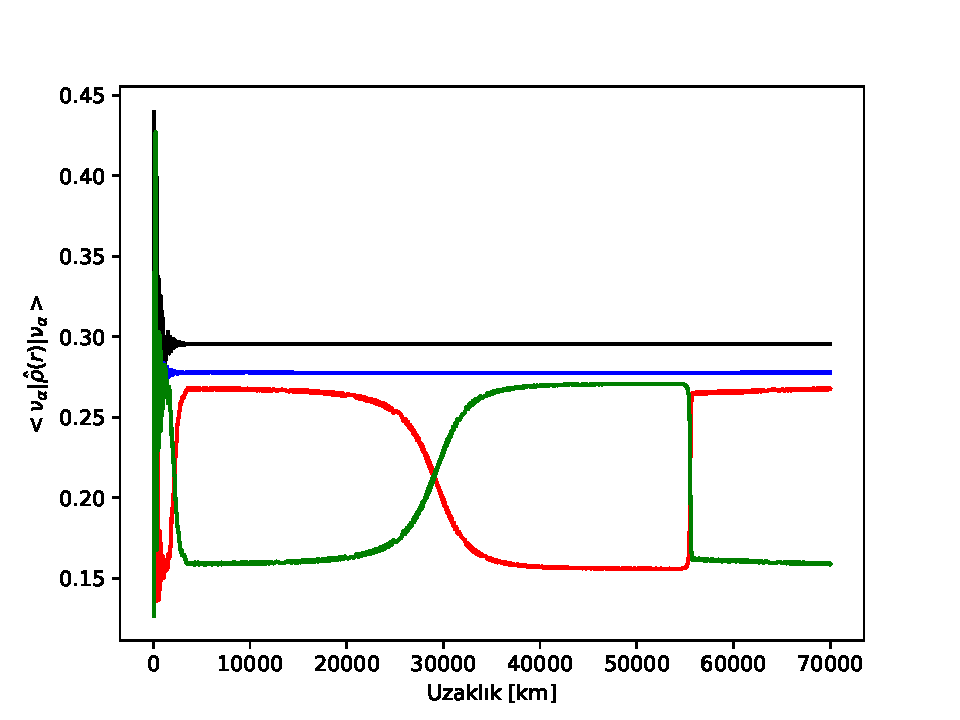
\includegraphics[width=0.9\textwidth]{figures/t5sCollnuB_distdiag10.pdf}
    \caption[t5sCollnuB Modeli, Yoğunluk Matrisinin Köşegen Elemanlarının Uzaklığa Göre Değişimi.]{t5sCollnuB Modeli, Yoğunluk Matrisinin Köşegen Elemanlarının Uzaklığa Göre Değişimi. Renk kodu: Siyah $ \nu_{e} $, mavi $ \nu_{x} $, kırmızı $ \nu_{\bar{e}} $, yeşil $ \nu_{\bar{x}} $}
    \label{fig:t5sCollnuB_distdiag10}
\end{figure}
\begin{figure}[hbt!]
    \centering
    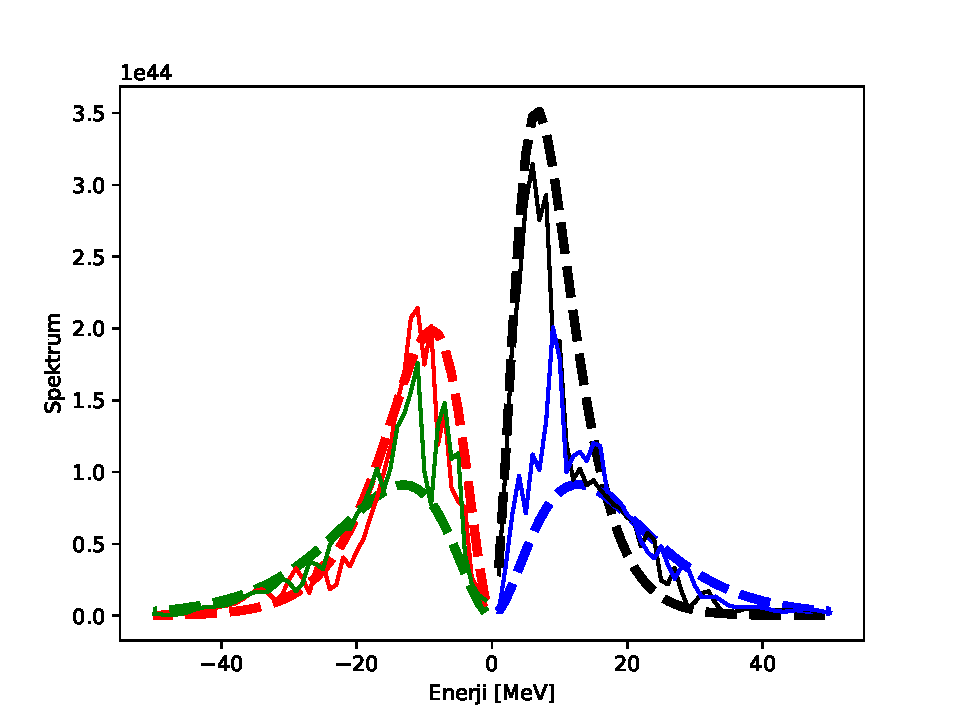
\includegraphics[width=0.9\textwidth]{figures/t5sCollnuB_spectrum.pdf}
    \caption[t5sCollnuB Modeli, Enerji Spektrumu.]{t5sCollnuB Modeli, Enerji Spektrumu. Renk kodu: Siyah $ \nu_{e} $, mavi $ \nu_{x} $, kırmızı $ \nu_{\bar{e}} $, yeşil $ \nu_{\bar{x}} $}
    \label{fig:t5sCollnuB_spectrum}
\end{figure}